\documentclass[12pt]{ucthesis}
%I removed natbib, deluxe table, bibsetup,lscape,
\usepackage{aasmacros,algorithm, algorithmic, amsmath, amsfonts,amssymb,amsthm,array,color,enumerate,epsfig,graphicx,longtable,multirow,psfrag}
\usepackage[pagebackref=true]{hyperref}
% \usepackage[font=normal,justification=raggedright,singlelinecheck=false]{caption}
\usepackage[caption=false,font=normal,justification=raggedright,singlelinecheck=false]{subfig}
\usepackage{fixltx2e}

\makeatletter
\@ifundefined{showcaptionsetup}{}{%
 \PassOptionsToPackage{caption=false}{subfig}}
\makeatother


\usepackage{longtable}
\usepackage{wrapfig}
\usepackage{calc}

%\usepackage{titlesec}
%\titlespacing*{\chapter}{0pt}{-50pt}{20pt}
%\titleformat{\chapter}[display]{\normalfont\huge\bfseries}{\chaptertitlename\ \thechapter}{20pt}{\Huge}
%\citestyle{aa}
\bibliographystyle{plain}
%% below needs to be after biliographystyle to make bib single-spaced
\usepackage{tweak_ucthesis}
\usepackage{todonotes}
\usepackage{amsthm}
\usepackage{listings}
% \usepackage{wrapfig}
% \usepackage{subfigure}				
\newcommand{\R}{\mathbb{R}}


\newtheorem{defn}{Definition}[section]
\newtheorem{proposition}{Proposition}[section]
\newtheorem{rem}{Remark}[section]
\newtheorem*{note}{Note}


\makeatletter

\global\long\def\modulo#1{{\left|#1\right|}}

\DeclareMathOperator{\sgn}{sgn}

\global\long\def\cvar{\rho}


\global\long\def\uptext{\text{U}}


\global\long\def\downtext{\text{D}}


\global\long\def\initvar#1{\bar{#1}}


\global\long\def\initstate{\initvar{\cvar}}


\global\long\def\dvar{\rho}


\global\long\def\initdiscrete{\initvar{\dvar}}


\global\long\def\discrete#1#2{\dvar_{#1}^{#2}}


\global\long\def\pfrac#1#2{\frac{\partial#1}{\partial#2}}


\global\long\def\Dfrac#1#2{\frac{d#1}{d#2}}


\global\long\def\links{\mathcal{I}}


\global\long\def\link{i}


\global\long\def\cind{j}


\global\long\def\nlinks{N}


\global\long\def\junctions{\mathcal{J}}


\global\long\def\jns{\junctions}


\global\long\def\junction{J}


\global\long\def\jn{\junction}


\global\long\def\RS{RS}


\global\long\def\convar{u}


\global\long\def\condiscrete#1#2{\convar_{#1}^{#2}}


\global\long\def\ncontrols{M}


\global\long\def\control{\vec{\convar}}


\global\long\def\state{\vec{\dvar}}


\global\long\def\density{\cvar}


\global\long\def\densitydiscrete#1#2{\discrete{#1}{#2}}


\global\long\def\defeq{:=}


\global\long\def\vect#1{\boldsymbol{\mathbf{#1}}}


\global\long\def\Inc{\text{Inc}}


\global\long\def\Out{\text{Out}}


\global\long\def\sys{H}


\global\long\def\syseq{h}


\global\long\def\cost{C}


\global\long\def\pmat#1#2{#1_{#2}}


\global\long\def\Hx{\pmat{\sys}{\state}}


\global\long\def\Hu{\pmat{\sys}{\control}}


\global\long\def\Jx{\pmat{\cost}{\state}}


\global\long\def\Ju{\pmat{\cost}{\control}}


\global\long\def\nominal#1{#1'}


\global\long\def\evaluate#1#2{\left.#1\right|_{#2}}


\global\long\def\tind{k}


\global\long\def\xind{j}


\global\long\def\ninc{n}


\global\long\def\nout{m}


\global\long\def\jlink#1#2{\link_{#1}^{#2}}


\global\long\def\jup#1{\jn_{#1}^{\uptext}}


\global\long\def\jdown#1{\jn_{#1}^{\downtext}}


\global\long\def\tuple#1#2{\left(#1,\ldots,#2\right)}


\global\long\def\trace#1{\hat{#1}}


\global\long\def\ntime{T}


\global\long\def\juncvar#1#2#3{\vec{#1}_{#2}^{#3}}


\global\long\def\juncstate#1#2{\juncvar{\dvar}{#1}{#2}}


\global\long\def\junctrace#1#2{\juncvar{\trace{\dvar}}{#1}{#2}}


\global\long\def\junccon#1#2{\juncvar{\convar}{#1}{#2}}


\global\long\def\ssvar{W_{R}}


\global\long\def\ss#1#2#3{\ssvar\left(#1;#2,#3\right)}


\global\long\def\god{g^{G}}


\global\long\def\ramp{\convar}


\global\long\def\length{L}


\global\long\def\intrange#1#2{\left\{  #1,\ldots,#2\right\}  }


% \global\long\def\degree#1{D_{#1}}


\global\long\def\demandsym{D}


\global\long\def\boundaryDemand#1#2{\demandsym_{#1}^{#2}}


\global\long\def\splitratio{\beta}


\global\long\def\barrierTerm{\epsilon}


\global\long\def\demand{\delta}


\global\long\def\rampDemand{d}


\global\long\def\supply{\sigma}


\global\long\def\ffspeed{v}


\global\long\def\congspeed{w}


\global\long\def\xdis#1{x_{#1}}


\global\long\def\fin#1#2{g_{#1,\uptext}^{#2}}


\global\long\def\fout#1#2{g_{#1,\downtext}^{#2}}


\global\long\def\framp#1#2{g_{#1,\downtext}^{#2}}

% \newcommand \noiseFactor \sigma

\makeatother
\newcommand{\dfract}[2]{\frac{d #1}{d #2}}
\newcommand{\vectorize}[1]{\mathbf{#1}}
\DeclareMathOperator*{\argmin}{arg\,min}
\renewcommand{\Re}{\mathbb{R}}

\newcommand{\augterm}{\psi}
\newcommand{\R}{\mathbb{R}}


\newtheorem{defn}{Definition}[section]
\newtheorem{proposition}{Proposition}[section]
\newtheorem{rem}{Remark}[section]
\newtheorem*{note}{Note}


\makeatletter

\global\long\def\modulo#1{{\left|#1\right|}}

\DeclareMathOperator{\sgn}{sgn}

\global\long\def\cvar{\rho}


\global\long\def\uptext{\text{U}}


\global\long\def\downtext{\text{D}}


\global\long\def\initvar#1{\bar{#1}}


\global\long\def\initstate{\initvar{\cvar}}


\global\long\def\dvar{\rho}


\global\long\def\initdiscrete{\initvar{\dvar}}


\global\long\def\discrete#1#2{\dvar_{#1}^{#2}}


\global\long\def\pfrac#1#2{\frac{\partial#1}{\partial#2}}


\global\long\def\Dfrac#1#2{\frac{d#1}{d#2}}


\global\long\def\links{\mathcal{I}}


\global\long\def\link{i}


\global\long\def\cind{j}


\global\long\def\nlinks{N}


\global\long\def\junctions{\mathcal{J}}


\global\long\def\jns{\junctions}


\global\long\def\junction{J}


\global\long\def\jn{\junction}


\global\long\def\RS{RS}


\global\long\def\convar{u}


\global\long\def\condiscrete#1#2{\convar_{#1}^{#2}}


\global\long\def\ncontrols{M}


\global\long\def\control{\vec{\convar}}


\global\long\def\state{\vec{\dvar}}


\global\long\def\density{\cvar}


\global\long\def\densitydiscrete#1#2{\discrete{#1}{#2}}


\global\long\def\defeq{:=}


\global\long\def\vect#1{\boldsymbol{\mathbf{#1}}}


\global\long\def\Inc{\text{Inc}}


\global\long\def\Out{\text{Out}}


\global\long\def\sys{H}


\global\long\def\syseq{h}


\global\long\def\cost{C}


\global\long\def\pmat#1#2{#1_{#2}}


\global\long\def\Hx{\pmat{\sys}{\state}}


\global\long\def\Hu{\pmat{\sys}{\control}}


\global\long\def\Jx{\pmat{\cost}{\state}}


\global\long\def\Ju{\pmat{\cost}{\control}}


\global\long\def\nominal#1{#1'}


\global\long\def\evaluate#1#2{\left.#1\right|_{#2}}


\global\long\def\tind{k}


\global\long\def\xind{j}


\global\long\def\ninc{n}


\global\long\def\nout{m}


\global\long\def\jlink#1#2{\link_{#1}^{#2}}


\global\long\def\jup#1{\jn_{#1}^{\uptext}}


\global\long\def\jdown#1{\jn_{#1}^{\downtext}}


\global\long\def\tuple#1#2{\left(#1,\ldots,#2\right)}


\global\long\def\trace#1{\hat{#1}}


\global\long\def\ntime{T}


\global\long\def\juncvar#1#2#3{\vec{#1}_{#2}^{#3}}


\global\long\def\juncstate#1#2{\juncvar{\dvar}{#1}{#2}}


\global\long\def\junctrace#1#2{\juncvar{\trace{\dvar}}{#1}{#2}}


\global\long\def\junccon#1#2{\juncvar{\convar}{#1}{#2}}


\global\long\def\ssvar{W_{R}}


\global\long\def\ss#1#2#3{\ssvar\left(#1;#2,#3\right)}


\global\long\def\god{g^{G}}


\global\long\def\ramp{\convar}


\global\long\def\length{L}


\global\long\def\intrange#1#2{\left\{  #1,\ldots,#2\right\}  }


% \global\long\def\degree#1{D_{#1}}


\global\long\def\demandsym{D}


\global\long\def\boundaryDemand#1#2{\demandsym_{#1}^{#2}}


\global\long\def\splitratio{\beta}


\global\long\def\barrierTerm{\epsilon}


\global\long\def\demand{\delta}


\global\long\def\rampDemand{d}


\global\long\def\supply{\sigma}


\global\long\def\ffspeed{v}


\global\long\def\congspeed{w}


\global\long\def\xdis#1{x_{#1}}


\global\long\def\fin#1#2{g_{#1,\uptext}^{#2}}


\global\long\def\fout#1#2{g_{#1,\downtext}^{#2}}


\global\long\def\framp#1#2{g_{#1,\downtext}^{#2}}

% \newcommand \noiseFactor \sigma

\makeatother
\newcommand{\dfract}[2]{\frac{d #1}{d #2}}
\newcommand{\vectorize}[1]{\mathbf{#1}}
\DeclareMathOperator*{\argmin}{arg\,min}
\renewcommand{\Re}{\mathbb{R}}

\newcommand{\augterm}{\psi}
\newcommand{\R}{\mathbb{R}}


\newtheorem{defn}{Definition}[section]
\newtheorem{proposition}{Proposition}[section]
\newtheorem{rem}{Remark}[section]
\newtheorem*{note}{Note}


\input{adjoint-commands}
\input{smart-america-commands}
\input{admm-commands}
\input{previous-articles/le/commands}
%\nofiles %% Uncomment for final edit of thesis.lof and thesis.lot

%% kluge to denote abstracts within thesis chapters
%\newcommand{\chabstract}{\medskip \bigskip {\bf \Large \centerline{Abstract} \bigskip}}
%% kluge to denote acknowledgements within thesis chapters
%\newcommand{\chacknowledgements}{\medskip \bigskip {\bf \Large \noindent Acknowledgements \bigskip \nopagebreak}}
%% kluge to fix figure/table numbers
%\renewcommand{\thefigure}{\thechapter.\arabic{figure}}
%\renewcommand{\thetable}{\thechapter.\arabic{table}}

%new command for theorems and all, the last bracket means to number within each chapter only
\newtheorem{remark}{Remark}[chapter]
%\renewcommand{\theremark}{\thechapter.\arabic{remark}}[chapter]
\newtheorem{prop}{Proposition}[chapter]
%\renewcommand{\theprop}{\thechapter.\arabic{prop}}
\newtheorem{definition}{Definition}[chapter]
%\renewcommand{\thedefinition}{\thechapter.\arabic{definition}}
\newtheorem{condition}{Condition}[chapter]
%\renewcommand{\thecondition}{\thechapter.\arabic{condition}}
\newtheorem{theorem}{Theorem}[chapter]
%\renewcommand{\thetheorem}{\thechapter.\arabic{theorem}}
\newtheorem{lem}{Lemma}[chapter]
\newtheorem{cor}{Corollary}[chapter]
\newtheorem{assumption}{Assumption}[chapter]
%\renewcommand{\thelemma}{\thechapter.\arabic{lemma}}

\let\originalleft\left
\let\originalright\right
\renewcommand{\left}{\mathopen{}\mathclose\bgroup\originalleft}
\renewcommand{\right}{\aftergroup\egroup\originalright}

%% if want to only compile parts
%\includeonly{frontmatter}
% \includeonly{le}
% \includeonly{security}
%~~~~~~~~~~~~~~~~~~~~~~~~~~~~~~~~~~~~~~~~~~~~~~~~~~~~~~~~~~~~~~~~~~~~~~~~~~~~~
\begin{document}
%~~~~~~~~~~~~~~~~~~~~~~~~~~~~~~~~~~~~~~~~~~~~~~~~~~~~~~~~~~~~~~~~~~~~~~~~~~~~~
%% declarations for front matter
\title{Optimization of Networked Dynamical Systems with Applications to Decentralized Freeway Control and Security of Traffic Systems}

%% go to bear facts to find your 'real' name
\author{Jack Daniel Reilly}

%% year you are getting this
\degreesemester{Fall}
\degreeyear{2014}

%% type of degree
\degree{Doctor of Philosophy}

%% committee chair
\chair{Professor Alexandre M. Bayen}

%% other committee members
\othermembers{
Professor Roberto Horowitz \\
Professor Scott Moura
}

%% total number of signers
\numberofmembers{3}

%% previous degrees (no longer needed, but need to designate as empty field)
\prevdegrees{}

%% main department
\field{Engineering -- Civil and Environmental Engineering}

%% campus
\campus{Berkeley}

%% make the title pages
\maketitle

%% copyright if you desire
\copyrightpage
\listoftodos

%% abstract
\begin{abstract}
This dissertation develops a general, scalable framework for controlling dynamical, networked systems based on mathematical optimization theory, with a strong focus on applications to freeway traffic management. The generality of the framework allows for controllers to consider high-level objectives applied to systems with complex, nonlinear dynamics.

A continuous freeway traffic model and its discretization was developed specifically for onramp metering control. The application serves as the motivating example behind the theory developed subsequently. To apply effective control on such systems, a discrete-adjoint-based \emph{model-predictive-control} (MPC) approach for controlling networked systems of conservation laws is presented, with explicit derivations for ramp metering applications. Linear scalability of the method with respect to network size and time horizon is derived for the discrete adjoint computations. To enable a more asynchronous control architecture, the dissertation presents a distributed optimization algorithm for dynamical, networked systems. The algorithm allows for a physical network to be partitioned into subnetworks that optimize locally and communicate only with adjacent subnetworks to achieve a globally optimal performance. 

Within the context of the \emph{Connected Corridors} project associated with UC Berkeley PATH, the developed theory was implemented in a production-level traffic management and simulation environment. Numerical examples applied to the San Diego I15 freeway are presented alongside the theory to motivate the highly practical aspects of the work. Simulations demonstrate the superiority of the MPC approach over existing methods widely used in practice.

The optimization tools are applied to an investigation of security and vulnerabilities of traffic control systems. The potential impact of a compromise of freeway traffic metering lights is analyzed using MPC and multi-objective optimization tools. Several realizable scenarios that exploit traffic system vulnerability locations are constructed and simulated to illustrate the severity of compromises.

Investigations are made into optimal rerouting strategies while controlling only a subset of network flow. A novel behavioral model is developed to account for the interaction of controllable and uncontrollable agents sharing a single flow network, where latency is a function of total flow. Using static freeway traffic models and communication network models, a framework based on convex optimization techniques is presented for computing rerouting policies, with numerical examples given for both freeway and communication networks.
\end{abstract}

%% begining of the front matter
\begin{frontmatter}
\renewcommand{\thepage}{\roman{page}}
\setcounter{page}{1}

%% dedication
\begin{dedication}
\null\vfil
{\large
\begin{center}
To Mom and Dad
\end{center}}
\null\vfil
\end{dedication}

%% TABLE OF CONTENTS
\tableofcontents
\listoffigures
\listoftables

%% if you want a 'list of code' when using the code/sty file, include these
%% %\listofcodes
%% %\addcontentsline{toc}{chapter}{List of Code Examples}
%% %

%% acknowledgements
\begin{acknowledgements}
% -*- root: thesis.tex -*-
I would first like to thank Professor Alexandre Bayen for inviting me into his lab five years ago and for working closely with me during the entirety of that time. From him I learned much about rigor, thoroughness, persuasiveness, leadership and professionalism: traits which I have found to be the most valuable assets gained during my PhD. I am forever grateful for his patience and guidance.

I would also like to thank Professor Roberto Horowitz, Dr. Gabriel Gomes, Dr. Ajith Muralidharan, and the other researchers in Professor Horowitz's lab. My work has benefited greatly from the different approaches to research and traffic in which I have participated. In particular, their work on linear formulations of freeway optimal control problems~\cite{gomes2006optimal,Muralidharana} greatly improved the practical nature of the theory developed within this thesis. Additionally, Gabriel's suggested extensions of my work to new problems such as network sensitivity analysis and model calibration have illuminated a broader applicability of the underlying research.

I give my gratitude to Professor Scott Moura, Professor Alexander Skabardonis, Professor Eli Yablonovitch, and Professor Steven Glaser for their guidance during my qualifying examination. Their feedback was valuable in directing the remainder of my research.


One of the most productive and enjoyable periods during my PhD was spent at the INRIA research center in Nice, France during Fall 2012, working with Dr. Paola Goatin and her student Maria Laura Delle Monache. I gained much insight into traffic models in general and how to develop a combined ordinary differential equation and partial differential equation model of freeway traffic. Their knowledge and methodology (e.g. mandatory coffee breaks) have permanently affected me.

I would also like to thank Raphael Marinier and Mihai Stroe of Google Road Traffic for their mentorship during my internship in Zurich, Switzerland in Summer 2013. Raphael's expertise in data analysis and focus on concrete results are skills I admire and attempt to emulate. I very much enjoyed the plethora of interesting traffic-related problems they have and their open-mindedness towards their solutions.

I thank again Professor Steven Glaser and thank Professor Raja Sengupta for welcoming me into the Civil Systems program mere days before the start of my Masters. Their novel approach to civil engineering is what reinvigorated my interest in the area, and I still regard my rash decision to switch into the Systems program as the best decision I have made.

I have had the pleasure to collaborate with many different students during my time in Berkeley. Specifically, I was lucky enough to work closely with Samitha Samaranayake over the last five years on many different projects and in many different venues (Sutardja Dai, La Val's, Nice, Tahoe, Gilman...). Additionally, I benefited greatly from the intelligence and philosophical musings of S\'{e}bastien Martin while working on freeway traffic security.

A distinguishing feature of my PhD was the ability to implement my research within production systems. I would like to thank Branko Kerkez and Mario Magliocco for their infinite patience with a greenhorn as I worked on the iShake project. I would also like to thank Joe Butler and many others, including Dimitris Triantafyllos, at CCIT and PATH for their dedication to supporting research in a professional environment and professionalism in a research environment.

To my dearest friends, Devon, Jack, Matty, Zack, Heidi, Timothy, Katelyn, thank you for embodying what I find good in this world.

Finally and foremost, I give my thanks and love to my mother Joanne, father Jim, and my brothers and best friends Jimmy and Christopher.
\end{acknowledgements}

\clearpage

\end{frontmatter}

\chapter{Introduction}
\label{sec:introduction}

\subsection{Motivation}
\label{sec:motivation}

\todo[inline]{lots of ``systems'' written here}

Modern physical systems, particularly those associated with public use such as freeway networks and water supplies, exist within a world with decreasing physical space and resources. For instance, freeways often cannot add additional lanes to accommodate increased demands. Thus, one must rely upon better managament systems and control algorithms in order to maximize performance within the limitations of the existing system. These ``smart'' systems make use of sensing instrumentation to estimate real-time conditions and modeling of the underlying physical dynamics to predict and plan for future states.

The focus of this thesis is the development of methods for the intelligent modeling and control of such networked dynamical systems. The goal is to provide operational managers with scalable, flexible, and robust algorithms that can leverage the well-instrumented and highly-connected control infrastructure present on modern systems. 

The remainder of this section discusses the \emph{Connected Corridors} project (Section~\ref{sec:connected-corridors}) on integrated freeway-corridor management (ICM), which served as the context in which this work was conducted, followed by an overview of \emph{model predictive control} (MPC) methods and their suitability in solving some of the main objectives put forth in the \emph{Connected Corridors} project (Section~\ref{sec:model-predictive-control}). The section concludes with a summary of the original contributions presented in this thesis (Section~\ref{sec:contributions}).

\subsection{Connected Corridors}
\label{sec:connected-corridors}

\emph{Connected-Corridors} is a project funded by the California Department of Transportation with the goal of creating the next generation of traffic management tools~\cite{connected-corridors,miller2010san}. While most current systems consider the freeway networks as independent from the city-street \emph{arterial} road networks, \emph{Connected Corridors} is tasked with creating an integrated approach to traffic management (referred to as ICM) which accounts for their dual performance. The project has demonstrated innovative control and estimation approaches to ICM on macroscopic and microscopic simulation environments (presented in Section~\ref{sec:numerical-results-adjoint}), with the ultimate plan of transferring the knowledge to a physical test-site within California.

The proposed ICM system possesses the following capabilities.

\begin{itemize}
	\item \textbf{Estimation}: Operators have access to a real-time estimation of the traffic conditions along the major freeways and adjacent arterials~\cite{work2010traffic,Jacqueta}.
	\item \textbf{Simulation}: Well-calibrated and efficient traffic models allow operators to simulate many different future traffic conditions~\cite{Muralidharan2009b,dervisoglu2014macroscopic}.
	\item \textbf{Control}: Traffic signal and message sign plans are computed online for many specialized objectives and serve as an optimized decision support tool~\cite{Reilly2013b,Reilly2014b}.
\end{itemize}

Control schemes implemented by the system include coordinated traffic light metering plans on freeway onramps (commonly referred as ramp metering, see Section~\ref{sec:continous-and-discrete-traffic-model-for-ramp-metering}) and traffic flow diversion around incidents via changeable message signs~\cite{Samaranayake2014}. 

\begin{figure}[htbp]
	\centering
	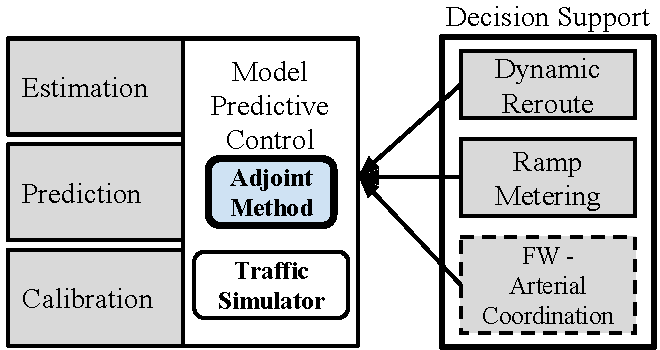
\includegraphics[width=0.8\textwidth]{diagrams/f2}
	\caption{\emph{Connected Corridors} control system architecture. The freeway state estimation, prediction and calibration submodules enable an MPC-based framework that computes coordinated, predictive decision-support strategies for numerous applications. Limited customization is required to extend the adjoint-based MPC controller to specific objectives or actuation types.}
	\label{fig:decision-support}
\end{figure}

To satisfy the above requirements, \emph{Connected Corridors} focuses on a number of submodules which are developed independently, but composed arbitrarily to create high-level, comprehensive support tools. Figure~\ref{fig:decision-support} shows a diagram of the several of the developed submodules and how they can be composed to create an MPC controller (explained in Section~\ref{sec:model-predictive-control}). Subsequently, the controller submodule is leveraged by a number of actuation strategies which have similar architectural requirements. For instance, both ramp metering and dynamic rerouting require real-time estimation and a calibrated freeway model to compute effective control strategies. Via submodule composition, much of the technology can be reused between the applications. This work contains the theory and implementation of constructing such controller submodules which efficiently exploit the structure of freeway networks.

\subsection{Model Predictive Control}
\label{sec:model-predictive-control}

Central to the \emph{Connected Corridors} approach of freeway traffic decision support is the concept of \emph{model predictive control} (MPC)~\cite{Muralidharana,o2013splitting,Frejo2011}. Generally speaking, MPC schemes successively compute a control policy which maximizes the performance, according to a provided criteria, of the system over the immediate future, where this work assumes the future to be of finite duration. The policy generated from the MPC scheme is recomputed as frequently as the real-time state estimation and computation times permit. Thus, associated with an MPC problem are two time periods: the \emph{update time} representing how often the MPC policy is recomputed online, and the \emph{time horizon} representing how far into the future for which the MPC policy will account. A more detailed treatment of MPC schemes is given in Section~\ref{sec:model-predictive-control-overview-adjoint-section}.

The requirements of an online MPC controller for a traffic system are depicted in Figure~\ref{fig:decision-support}. At the base of the method is a mathematical model of the physical system, referred to as the \emph{forward system}. These models often require calibration using historical sensor measurements to set the model parameters. To fully specify the simulation, an \emph{initial condition} is specified (i.e. estimation), as well as the \emph{boundary conditions} at the exteriors of the system over the entire time horizon of the MPC problem (i.e. prediction). All these requirements are satisfied by componenets within the \emph{Connected Corridors} system~\cite{Muralidharan2009b,dervisoglu2014macroscopic,work2010traffic}, making MPC control a natural fit for research and development in the project.

The focus of this thesis is the efficient and flexible design of MPC optimization techniques and their applications to freeway control systems. At the heart of the developed approach is the \emph{discrete adjoint} method for gradient computations within first-order gradient descent methods (Section~\ref{chapter:adjoint}). The efficiency of the developed method enables \emph{online} application of MPC to the control of large freeway networks (on the order of tens of miles) with frequent recomputations (on the order of one minute) to ``close the loop'' with real-time measurements.

\subsection{Contributions}
\label{sec:contributions}

This thesis contains the following contributions to the problem of optimal control of networked dynamical systems.

\begin{itemize}
	\item \textbf{A novel continuous freeway traffic model suitable for finite-horizon optimal control problems}~\cite{delle2014pde,Reilly2013b}.
	\begin{itemize}
		\item The model represents an extension of the networked \emph{Lighthill-Richards-Whitham} (LWR) PDE traffic model~\cite{lighthill1955kinematic,richards1956shock} proposed in~\cite{garavello2006traffic}, where onramps are modeled as ODE buffers to guarantee \emph{strong} boundary conditions and flow conservation at the network boundaries.
		\item A discretized version of the continuous model is derived for optimal control application using Godunov's method~\cite{godunov1959,lebacque1996godunov}.
	\end{itemize}
	\item \textbf{A method for optimal control of networked conservation law systems based on discrete adjoint calculations}~\cite{Reilly2013b,Samaranayake2014}.
	\begin{itemize}
		\item This work develops a framework for converting a continuous time and space control problem on a physical network, where edges behave according to a conservation law, into a discrete, finite-horizon optimal control problem using Godunov discretization.
		\item The application of the discrete adjoint method~\cite{Giles2000,Duffy2009,d2010modeling,Gugat2005} to compute gradients for the above problem is presented, with an analysis of the linear scalability of the approach in discrete time and discrete space for sparse network structures.
		\item An explicit formulation of the discrete adjoint method is given for the application of coordinated ramp metering control~\cite{Papageorgiou1991,Frejo2011,Kotsialos2004,gomes2006optimal} for freeway networks.
		\item MPC numerical simulations on a macroscopic model of the I15 South Freeway in San Diego, California demonstrate the practical nature and the robustness to measurement noise of the research.
	\end{itemize}
	\item \textbf{A decentralized algorithm and control infrastructure for networked dynamical systems}~\cite{Reilly2014b}.
	\begin{itemize}
		\item This thesis presents a new distributed optimization method based on the alternating directions methods of multipliers (ADMM)~\cite{Boyd2010a,gabay1976dual,mota2012distributed} algorithm for solving  optimal control problems over subnetworks in parallel. The splitting method is done in such a way to only require communication between physically-neighboring subnetworks.
		\item Differing from similar work where subsystems only share control variables~\cite{mota2012distributed,camponogara2009distributed}, the presented method allows for subsystems to share both control \emph{and state} variables, an assumption necessary for the distributed control of traffic networks and hydrological systems.
		\item A discrete adjoint formulation is presented for efficient solution of subsystems with coupled control and state variables.
	\end{itemize}
	\item \textbf{An analysis of the security of traffic control systems and coordinated ramp metering attacks}~\cite{Reilly2014c,Reilly2014a}.
	\begin{itemize}
		\item A classification of traffic system vulnerability locations is constructed across such categories as cost of attack, effectivenes, and directness of control.
		\item A novel analysis of the potential damage and impact of coordinated ramp metering attacks is conducted using adjoint-based optimal control and multi-objective optimization tools.
		\item Illustrative attack scenarios are constructed and numerically investigated on realistic freeway networks. A web-based coordinated ramp metering attack tool was created to implement the interactive optimization approaches presented in the work~\cite{smartroadswebsite}.
	\end{itemize}
\end{itemize}

\subsection{Organization}
\label{sec:organization}

The rest of the article is organized as follows.

Chapter~\ref{chapter:freeway-network-model} presents the continuous and discrete freeway models which serves as the running application of the theory presented subsequently.  After convering preliminaries on networked PDE systems, the derivation of and motivation behind the model are given.

Chapter~\ref{chapter:adjoint} presents the discrete adjoint approach to optimal control of networked conservation laws. Presented first is a general overview of the discrete adjoint method, followed by its specific instantiation for discretized physical network systems. The application to coordinated ramp metering is then presented with numerical examples. The chapter concludes with the distributed, asynchronous formulation of the adjoint optimal control method via subnetwork splitting.

Chapter~\ref{chapter:security} presents a study of traffic control systems and their vulnerabilities. After defining the specific control system under consideration and its security weaknesses, the work gives an in-depth study of coordinated ramp metering attacks.

Finally, we conclude with a overview of the work presented, as well as directions for future research.
\chapter{Freeway Network Model}
\label{chapter:freeway-network-model}

\section{Preliminaries of Networked Conservation Laws}

\subsection{Networked Conservation Laws}

\subsection{Riemann Solvers}

\subsection{Godunov Discretization}

\section{Continuous and Discrete Traffic Model for Ramp Metering}
\label{sec:continous-and-discrete-traffic-model-for-ramp-metering}

\subsection{Overview on Traffic Models and Ramp Metering}

\subsection{LWR Equation}

\subsection{Flow Conservation at Network Boundaries}

\subsection{Continuous PDE-ODE Freeway Model}

\subsection{Discrete Freeway Model}
%!TEX root = restart.tex
\section{Adjoint Based Flow Optimization\label{sec:Adjoint-method}}

In  this section, we propose a discrete adjoint approach to compute optimal ramp-metering stategies on road networks modeled by conservation laws.
Networks of one-dimensional conservation laws,
described by systems of nonlinear first-order hyperbolic \textit{partial
differential equations}~(PDEs), are an efficient framework for modeling
physical phenomena, such as freeway traffic evolution~\cite{garavello2006traffic,work2010traffic,frazzoli2002real} and supply
chains~\cite{Brunnermeier1999}. Similarly, PDE systems of balance laws are useful in modeling gas pipeline flow~\cite{Gugat2011Gas,Rothfarb1970Optimal} and water channels~\cite{Gugat2012Contamination,Rabbani2010}. Optimization
and  control of these networks is an active field of
research~\cite{Gugat2005,Bayen2006,Kotsialos2004}. More generally, numerous
techniques exist for the control of conservation laws, such as, for example,
backstepping~\cite{Coron2013,Glass2007}, Lyapunov-based methods~\cite{Coron2013}, and
optimal control methods~\cite{Jacquet2006,Blanchard2013,Keller2013}.
In particular, a common  approach is to compute the gradient of the cost functional via the \textit{adjoint method}~\cite{Giles2000Introduction,Jameson2000Aerodynamic,Raffard2008}.
Nevertheless, its implementation in the framework of nonlinear conservation laws presents several difficulties linked to the discontinuous  character of the solutions. In particular, the presence of shocks in the solutions requires a careful sensitivity analysis based on the use of shift-differentials and generalized tangent vectors, see~\cite{Bressan1997ShiftDifferentiability,Ulbrich2002Sensitivity,Ulbrich2003AdjointBased}.

Extensive study has also been conducted on the choice of method for effectively computing the gradient via the adjoint. In particular, the continuous adjoint
method~\cite{Jacquet2005,Gugat2005,Moin1994,Reuther1996} operates directly on
the PDE and a so-called adjoint PDE system, which when solved can be used to
obtain an explicit  expression of the gradient of the underlying optimization
problem. Conversely,  the discrete adjoint
method~\cite{Giles2000,Gugat2005,Kotsialos2004} first discretizes a
continuous-time PDE and then requires the solution of a set of linear
equations  to solve for the gradient. Finally, a third approach exists, which
uses  automatic differentiation techniques to automatically generate an
adjoint  solver from the numerical representation of the forward
system~\cite{Muller2005,Giering1998}.

It is well known that the numerical treatment of the adjoint method imposes a careful choice of the discretization scheme to avoid the introduction of numerical errors  at discontinuities~\cite{Giles2003Discrete}.
Rigorous convergence results for optimization problems have been provided for Lax-Friedichs type schemes~\cite{Giles2010Convergencea} and relaxation methods~\cite{Banda2012Adjoint}.
The case of road networks in free flow conditions is addressed in~\cite{Gugat2005}.
In our more general setting of PDE networks and applications to freeway traffic control, the presence of junction conditions with both forward and backward-moving shockwaves led us the use of a modified Godunov scheme that precisely takes into account the flows at the network nodes. An alternative approach involves using Lax-Friedichs-type discretizations with higher-resolution interpolation schemes~\cite{Nessyahu1990NonOscillatory}. Moreover, general existence and stability results for the corresponding system of equations modeling traffic evolution on the network are still missing at the moment.
Therefore, establishing rigorous convergence results for the gradient computation in this framework is out of the scope of this thesis. Here we made the choice of the discrete adjoint approach, which derives the gradient directly from the discretized system, thus avoiding dealing with weak boundary conditions in the continuous system~\cite{garavello2006traffic,work2010traffic,strub2006weak}.

% we could use a variant of the lax-friedrichs.
% goettlich, staggered lax-friedrichs, to have a more precise approximation, lax friedrichs is very diffusive.





%While the continuous adjoint formulation results in a compact formulation, 
%better intuition into the system's sensitivities with respect to the objective, 
%and well-posedness of the control's solution (when it can be proved), it is 
%often difficult to derive for systems of hyperbolic nonlinear PDEs controlled 
%by boundary conditions, when these boundary conditions have to be written in the 
%weak sense.
%Additionally, the continuous adjoint must eventually be discretized in order to 
%produce numerical solutions for the optimization problem. Finally, the 
%differentiation of the forward PDE is sometimes problematic due to the lack of 
%regularity of the solution~\cite{garavello2006traffic,work2010traffic} which 
%makes the formal definition of the adjoint problem more difficult.
%The discrete adjoint approach derives the gradient directly from the 
%discretized system, thus avoiding working directly with weak boundary 
%conditions in the continuous 
%system~\cite{garavello2006traffic,work2010traffic,strub2006weak}.
%Automatic differentiation techniques can simplify the repetitive 
%steps of the discrete adjoint derivation, but sometimes at the cost of 
%sub-optimal code implementations with respect to memory and CPU 
%consumption~\cite{Giles}. A more-detailed analysis of the trade-offs associated 
%with each method is given in~\cite{Giles}.

There exist many applications of the adjoint method for control, optimization 
and estimation of physical systems in engineering. Shape optimization of 
aircraft~\cite{Reuther1996,Giles1997,Moin1994} has applied the method 
effectively to reduce the computational cost in gradient methods associated 
with the large number of optimization parameters. The technique has also been 
applied in parameter identification of biological systems~\cite{Raffard2008}. 
State estimation problems can be phrased as optimal control problems by setting 
the unknown state variables as control parameters and penalizing errors in 
resulting state predictions from known values. This approach has been applied 
to such problems as open water state estimation~\cite{Castaings2006,Strub2009} 
and freeway traffic state estimation~\cite{Jacqueta}.

Since conservation laws may be nonlinear by nature and lead to non-convex or 
nonlinear formulations of the corresponding optimization problem, fewer 
efficient optimization techniques exist for the 
discretized version of these problems than for convex problems for example. One 
approach is to approximate the system with a ``relaxed'' version in order to 
use efficient linear programming techniques. In transportation, by 
relaxing the Godunov discretization scheme, the linearization approach was used 
in~\cite{gomes2006optimal} for optimal ramp metering, and 
in~\cite{ziliaskopoulos2000linear} for optimal route assignment which is exact 
when the relaxation gap can be shown to be zero. The ramp 
metering technique in~\cite{Muralidharana} uses an additional control parameter 
(variable speed limits) to mimic the linearized freeway dynamics. While the 
upside of these methods is reduced computational complexity and the guarantee 
of finding a globally optimal solution, the downside is that the model of the 
linearized physical system may greatly differ from the actual system to which 
the control policies would be applied.

Another approach avoids discretization of the continuous system by taking advantage of certain simplifying assumptions in the dynamics. In~\cite{Fugenschuh2006Combinatorial}, the problem of finding optimal split ratios on a traffic networks is efficiently solved by deriving non-linear and linear algebraic formulations of a simplified form of the continuous system dynamics which only considers forward-moving shockwaves. In~\cite{Apice2010Modeling}, a mixed-integer linear program (MILP) formulation is posed for the optimal routing of goods on a supply chain, leading to efficient solutions of this particular application. The number of integer constraints needed in the MILP formulation is proportional to the number of non-linear constraints in the underlying system and has a direct impact on the efficiency of MILP solvers. Applications to highly non-linear systems such as freeway traffic may prefer non-linear programming approaches such as the adjoint method using non-linear discretization techniques, which avoid integer constraints and allow the constraints to capture more complex dynamics.

Alternatively, nonlinear optimization techniques can be applied to the 
discretized system without any modification to the underlying dynamics. This 
approach leads to more expensive optimization algorithms, such as gradient 
descent, and no guarantee of finding a global optimum. One difficulty in this 
approach comes in the computation of the gradient, which, if using finite 
differences, requires a full forward-simulation for each perturbation of a 
control parameter. This approach is taken in~\cite{Ramon2013,Frejo2011} to 
compute several types of decentralized ramp metering strategies. The increased 
complexity of the finite differences approach for each additional control 
parameter makes the method unsuitable for real-time application on 
moderately-sized freeway networks.

Ramp metering is a common freeway control strategy, providing a means of 
dynamically controlling freeway throughput without directly impeding mainline 
flow or implementing complex tolling systems. While metering strategies have 
been developed using microscopic models~\cite{Ben-Akiva2003}, most strategies 
are based off macroscopic state parameters, such as vehicle density and the 
density's relation to 
speed~\cite{richards1956shock,lighthill1955kinematic,daganzo1995cell}. Reactive 
metering strategies~\cite{Papageorgiou1991Alinea,Papamichail,Kachroo2003} use 
feedback from freeway loop detectors to target a desired mainline density, 
while predictive metering 
strategies~\cite{Frejo2011,Kotsialos2004,gomes2006optimal,Chen1997} use a 
physical model with predicted boundary flow data to generate policies over a 
finite time horizon. Predictive methods are often embedded within a model 
predictive control loop to handle uncertainties in the boundary data and 
cumulative model errors~\cite{Muralidharana}.

This article develops a framework for efficient control of discretized 
conservation law PDE networks using the adjoint 
method~\cite{Giles2000,Pironneau1974} via Godunov 
discretization~\cite{godunov1959}, while detailing its application to 
coordinated ramp metering on freeway networks. Note that the method can be 
extended without significant difficulty to other numerical schemes commonly 
used to discretize hyperbolic PDEs. We show how the complexity of 
the gradient computation in nonlinear optimal control problems can be greatly 
decreased by using the discrete adjoint method and exploiting the decoupling 
nature of the problem's network structure, leading to efficient gradient 
computation methods. After giving a general framework for computing the gradient 
over the class of scalar conservation law networks, we show that the system's 
partial derivatives have a sparsity structure resulting in gradient computation 
times linear in the number of state and control variables for networks of small 
vertex degree. Memory usage is also linear when sparse data structures are utilized. The results are 
demonstrated by running a coordinated ramp metering strategy on a 19 mile 
freeway stretch in California faster than real-time, while giving traffic 
performance superior to that of state of the art practitioners tools.

The rest of the section is organized as follows. 
Section~\ref{sec:Preliminaries} gives an 
overview of scalar conservation law networks and their discretization via the 
Godunov method, while introducing the nonlinear, finite-horizon optimal control 
problem. Section~\ref{sec:Adjoint-method} details the adjoint method derivation 
for this class of problems and shows how it can be used to compute the gradient 
in linear time in the number of discrete state and control variables.  
Section~\ref{sec:Applications-to-Optimal} shows how the adjoint method can be 
applied to the problem of optimal coordinated ramp metering, with numerical 
results on a real freeway network in California shown in 
Section~\ref{sec:Numerical-results-for}. Finally, some concluding remarks are 
given in Section~\ref{sec:Conclusions}.


\subsection{Optimal Control Problem Formulation\label{par:Optimization-Problem}}

In addition to our governing equations $\sys\left(\state,\control\right)=0$, where we assume each $h_i^k \in \mathcal{C}^1$,
we also introduce a cost function $\cost \in \mathcal{C}^1$.

\begin{eqnarray*}
\cost: & \mathbb{R}^{\nlinks T}\times\mathbb{R}^{\ncontrols T} & \rightarrow\mathbb{R}\\
& \left(\state,\control\right) & \mapsto\cost\left(\state,\control\right)
\end{eqnarray*}
which returns a scalar that serves as a metric of performance of the
state and control values of the system. We wish to minimize the quantity
$\cost$ over the set of control parameters $\control$, while constraining
the state of the system to satisfy the governing equations $\sys\left(\state,\control\right)=0$,
which is, again, the concatenated version of~\eqref{eq:main-ge} or~\eqref{eq:syseq-god}.
We summarize this with the following optimization problem:

\begin{eqnarray}
\underset{\control}{\min} & \cost\left(\state,\control\right)\nonumber \\
\text{subject to:} & \sys\left(\state,\control\right)=0\label{eq:op-problem}
\end{eqnarray}
Both the cost function and governing equations may be non-convex in
this problem.


\subsection{Calculating the Gradient\label{par:Calculating-the-gradient}}

We wish to use gradient information in order to find control values
$\control^{*}$ that give locally optimal costs $\cost^{*}=\cost\left(\state\left(\control^{*}\right),\control^{*}\right)$.
Since there may exist many local minima for this optimization problem~\eqref{eq:op-problem}
(which is non-convex in general), gradient\emph{ }methods do not guarantee
global optimality of $\control^{*}$\emph{. }Still, nonlinear optimization
methods such as interior point optimization utilize gradient information
to improve performance~\cite{Andreas2005}.

In a descent algorithm, the optimization procedure will have to descend
a cost function, by coupling the gradient, which, at a nominal point
$\left(\nominal{\state},\nominal{\control}\right)$ is given by:

\begin{equation}
d_{\control}\cost\left(\nominal{\state},\nominal{\control}\right)=\evaluate{\pfrac{\cost\text{\ensuremath{\left(\state,\control\right)}}}{\state}}{\nominal{\state},\nominal{\control}}\Dfrac{\state}{\control}+\evaluate{\pfrac{\cost\text{\ensuremath{\left(\state,\control\right)}}}{\control}}{\nominal{\state},\nominal{\control}}\label{eq:j-v}.
\end{equation}

\begin{note}
For Equation~\eqref{eq:j-v} to be valid, all required partial and full derivatives must be well-defined, including $\Dfrac{\state}{\control}$. In some applications, this assumption does not necessarily hold,
either because $f$ itself is not smooth or because $\god$ is not
smooth (and thus $H \notin \mathcal{C}^1$), as is the case for the LWR equation with concave fundamental diagrams. There are several settings in which the
conditions for differentiability are satisfied, see in particular~\cite{Gugat2005,Flasskamp2012}.
\end{note}

The main difficulty is to compute the term $\Dfrac{\state}{\control}$.
We take advantage of the fact that the derivative of $H\left(\state,\control\right)$
with respect to $\control$ is equal to zero along trajectories of
the system:

\begin{equation}
d_{\control}\sys\left(\nominal{\state},\nominal{\control}\right)=\evaluate{\pfrac{\sys\text{\ensuremath{\left(\state,\control\right)}}}{\state}}{\nominal{\state},\nominal{\control}}\Dfrac{\state}{\control}+\evaluate{\pfrac{\sys\text{\ensuremath{\left(\state,\control\right)}}}{\control}}{\nominal{\state},\nominal{\control}}=0\label{eq:h-v}.
\end{equation}


The partial derivative terms, $\Hx\in\mathbb{R}^{\nlinks\ntime\times\nlinks\ntime}$,
$\Hu\in\mathbb{R}^{\nlinks\ntime\times\ncontrols\ntime}$, $\Jx\in\mathbb{R}^{\nlinks\ntime}$,
and $\Ju\in\mathbb{R}^{\ncontrols\ntime}$, can all be evaluated (more
details provided in Section~\ref{sub:Evaluating--and}) and then
treated as constant matrices. Thus, in order to evaluate $d_{\control}\cost\left(\nominal{\state},\nominal{\control}\right)\in\mathbb{R}^{\ncontrols\ntime}$,
we must solve a coupled system of matrix equations.

\paragraph{Forward system.\label{par:Forward-system}}

If we solve for $\Dfrac{\state}{\control}\in\mathbb{R}^{\nlinks\ntime\times\ncontrols\ntime}$
in~\eqref{eq:h-v}, which we call the \emph{forward system}:

\[
\Hx\Dfrac{\state}{\control}=-\Hu,
\]
then we can substitute the solved value for $\Dfrac{\state}{\control}$
into~\eqref{eq:j-v} to obtain the full expression for the gradient.
Section~\ref{sub:Evaluating--and} below gives details on the invertibility
of $\Hx$, guaranteeing a solution for $\Dfrac{\state}{\control}$.


\paragraph{Adjoint system.\label{par:Adjoint-system}}

Instead of evaluating $\Dfrac{\state}{\control}$ directly, the adjoint
method solves the following system, called the adjoint system,
for a new unknown variable $\lambda\in\mathbb{R}^{\nlinks\ntime}$
(called the adjoint variable):

\begin{equation}
\Hx^{T}\lambda=-\Jx^{T}\label{eq:adjoint}
\end{equation}

Under certain additional conditions on the flux function and discretization scheme, the adjoint system in Equation~\eqref{eq:adjoint} may be shown to converge to the continuous adjoint system as the discretization steps go towards zero, as described in the following works~\cite{Ulbrich2003AdjointBased,Banda2012Adjoint,Gugat2005}. No such convergence results exist in our setting of using a Godunov discretization with general $n\times m$ junctions.

The expression for the gradient becomes:

\begin{equation}
d_{\control}\cost\left(\nominal{\state},\nominal{\control}\right)=\lambda^{T}\Hu+\Ju\label{eq:adjoint-grad}
\end{equation}

We note that Equations~\eqref{eq:adjoint} and~\eqref{eq:adjoint-grad} can be alternatively derived using the first-order \emph{Karush-Kuhn-Tucker} (KKT) conditions, coupled with the constraint qualification in Equation~\eqref{eq:op-problem}. Given the assumed non-convexity of the underlying system, first-order KKT conditions are necessary, but not sufficient conditions for optimality of $\mathbf{\control}$ and $\lambda$. For practical applications to non-convex systems and for the purposes of this article, we do not necessarily seek global \emph{or local} optimality, but rather the direction of steepest descent given in Equation~\eqref{eq:adjoint-grad} in order to \emph{improve} the performance of the system.

We define $\degree{\state}$ to be the maximum junction degree on
the network:

\begin{equation}
\degree{\state}=\max_{\jn\in\jns}\left(\ninc_{\jn}+\nout_{\jn}\right),\label{eq:dx}
\end{equation}
and also define $\degree{\control}$ to be the maximum number of constraints
that a single control variable appears in, which is equivalent to:

\begin{equation}
\degree{\control}=\max_{\condiscrete{}{}\in\control}\sum_{\jn\in\jns:\condiscrete{}{}\in\junccon{\jn}{\tind}}\left(\ninc_{\jn}+\nout_{\jn}\right)\label{eq:dv}.
\end{equation}


Note that $\left\{ \convar\in\junccon{\jn}{\tind}:\jn\in\jns\right\} $
is a $\tind$-dependent set. By convention, junctions are either actuated
or not, so there is no dependency on $\tind$, i.e. if $\exists\tind$
s.t. $\convar\in\junccon{\jn}{\tind}$, then $\forall\tind$, $\convar\in\junccon{\jn}{\tind}$.

Using these definitions, we show later in Section~\ref{sub:Complexity-of-solving}
how the complexity of computing the gradient is reduced from $O(\degree{\state}\nlinks\ncontrols\ntime^{2})$
to $O(\ntime\left(\degree{\state}\nlinks+\degree{\control}\ncontrols\right))$
by considering the adjoint method over the forward method.

\begin{figure}
\begin{centering}
\subfloat[\label{fig:genneta}]{\begin{centering}
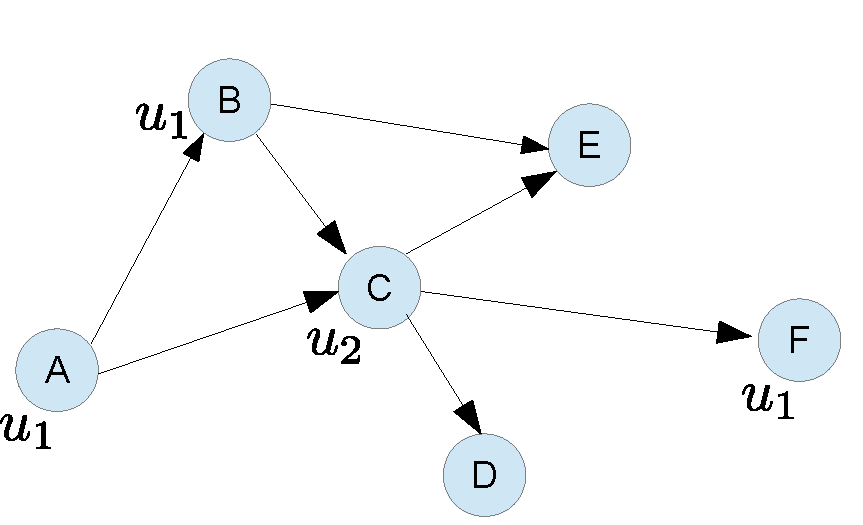
\includegraphics[width=0.33\columnwidth]{figs-gen/gen-net}
\par\end{centering}

}\subfloat[\label{fig:gennetb}]{\begin{centering}
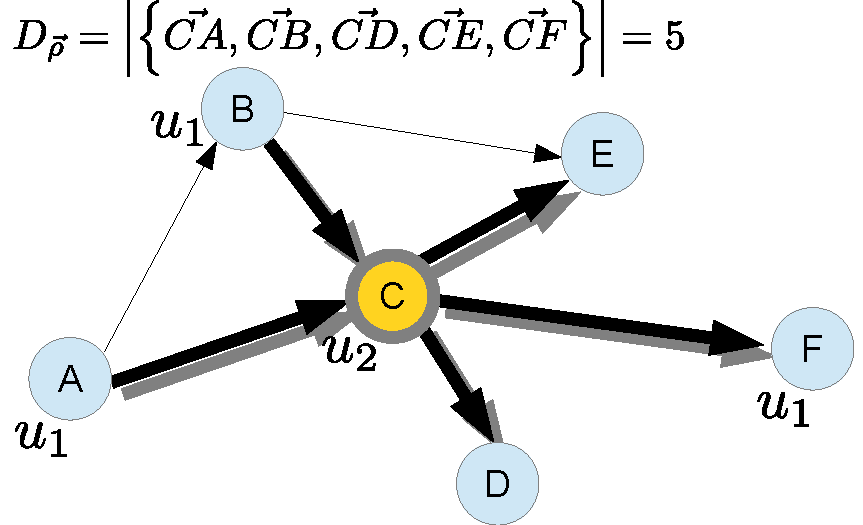
\includegraphics[width=0.33\columnwidth]{figs-gen/gen-net-dx}
\par\end{centering}

}\subfloat[\label{fig:gennetc}]{\begin{centering}
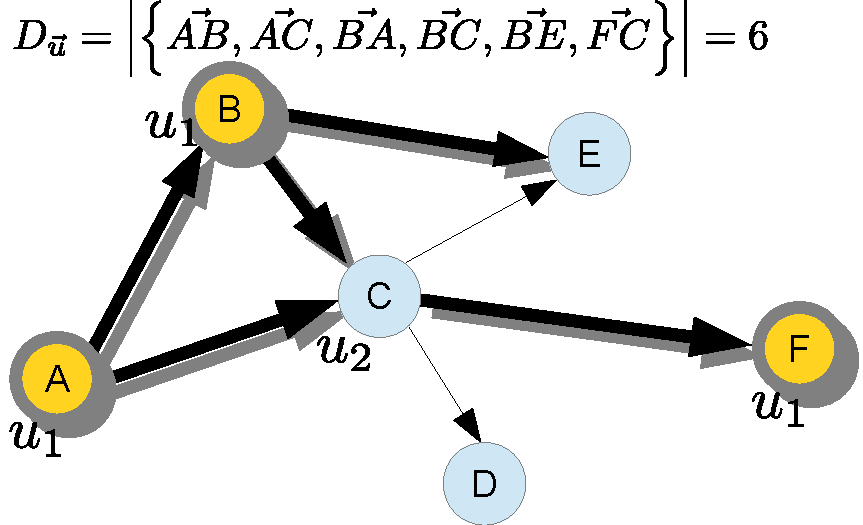
\includegraphics[width=0.33\columnwidth]{figs-gen/gen-net-dv}
\par\end{centering}

}
\par\end{centering}

\caption{Depiction of $D_{\state}$ and $D_{v}$ for an arbitrary graph. Fig.~\ref{fig:genneta}
shows the underlying graphical structure for an arbitrary PDE network.
Some control parameter $\convar_{1}$ has influence over junctions
$A$, $B$, and $F$, while another control parameter $\convar_{2}$
has influence over only junction $C$. Fig.~\ref{fig:gennetb}
depicts the center junction having the largest number of connecting
edges, thus giving $D_{\state}=5$. Fig.~\ref{fig:gennetc} shows
that control parameter $\convar_{1}$ influences three junctions with
sum of junctions degrees equal to six, which is maximal over the other
control parameter $\convar_{2}$. leading to the result $D_{\control}=6$.
Note that in Fig.~\ref{fig:gennetc}, the link going from junction
$A$ to junction $B$ is counted twice: once as an outgoing link $\vec{AB}$
and once as in incoming link $\vec{BA}$.\label{fig:Depicting--and}}
\end{figure}

A graphical depiction of $D_{\state}$ and $D_{\control}$ are given
in Fig.~\ref{fig:Depicting--and}. Freeway networks are usually considered to have topologies that are
nearly planar, leading to junctions degrees which typically do not
exceed 3 or 4, regardless of the total number of links. Also, from
the locality argument for control variables in Section~(\ref{sec:State,-control,-and}),
a single control variable's influence over state variables will not
grow with the size of the network. Since the $\degree{\state}$ and
$\degree{\control}$ typically do not grow with $\nlinks\ntime$ or
$\ncontrols\ntime$ for freeway networks, the complexity of evaluating
the gradient for such networks can be considered linear for the adjoint
method.


\subsection{Evaluating the Partial Derivatives\label{sub:Evaluating--and}}

While no assumptions are made about the sparsity of the cost function
$\cost$, the networked-structure of the PDE system and the Godunov
discretization scheme allows us to say more about the structure and
sparsity of $\Hx$ and $\Hu$.


\paragraph{Partial derivative expressions.}

Given that the governing equations require the evaluation of a Riemann
solver at each step, we detail some of the necessary computational
steps in evaluating the $\Hx$ and $\Hu$ matrices. 

If we consider a particular governing equation $\syseq_{\link}^{\tind}\left(\state,\control\right)=0$,
then we may determine the partial term with respect to $\discrete jl\in\state$
by applying the chain rule:

\begin{align}
\pfrac{\syseq_{\link}^{\tind}}{\discrete jl}=\pfrac{\discrete{\link}{\tind}}{\discrete jl}-\pfrac{\discrete{\link}{\tind-1}}{\discrete jl} & +\frac{\Delta t}{L_{i}}f'\left(\RS_{\jdown{\link}}\left(\juncstate{\jdown{\link}}{\tind-1},\junccon{\jdown{\link}}{\tind-1}\right)_{\link}\right)\pfrac{}{\discrete jl}\left(\RS_{\jdown{\link}}\left(\juncstate{\jdown{\link}}{\tind-1},\junccon{\jdown{\link}}{\tind-1}\right)_{\link}\right)\label{eq:dhdufull} \\
& -\frac{\Delta t}{L_{i}}f'\left(\RS_{\jup{\link}}\left(\juncstate{\jup{\link}}{\tind-1},\junccon{\jup{\link}}{\tind-1}\right)_{\link}\right)\pfrac{}{\discrete jl}\left(\RS_{\jup{\link}}\left(\juncstate{\jup{\link}}{\tind-1},\junccon{\jup{\link}}{\tind-1}\right)_{\link}\right)\nonumber                       
\end{align}				
or if we consider the composed Riemann flux solver $\god_{\jn}$ in~\eqref{eq:god-jn}:

\begin{equation}
\pfrac{\syseq_{\link}^{\tind}}{\discrete jl}=\pfrac{\discrete{\link}{\tind}}{\discrete jl}-\pfrac{\discrete{\link}{\tind-1}}{\discrete jl}+\frac{\Delta t}{L_{i}}\left(\pfrac{}{\discrete jl}\left(\god_{\jdown{\link}}\left(\juncstate{\jdown{\link}}{\tind-1},\junccon{\jdown{\link}}{\tind-1}\right)\right)_{\link}-\pfrac{}{\discrete jl}\left(\god_{\jup{\link}}\left(\juncstate{\jup{\link}}{\tind-1},\junccon{\jup{\link}}{\tind-1}\right)\right)_{\link}\right)\label{eq:dhdugod}
\end{equation}


A diagram of the structure of the $\Hx$ matrix is given in Fig.~(\ref{fig:partial-ordering}).
\begin{figure}
\subfloat[\label{fig:partial-ordering}Ordering of the partial derivative terms.
Constraints and state variables are clustered first by time, and then
by cell index.]{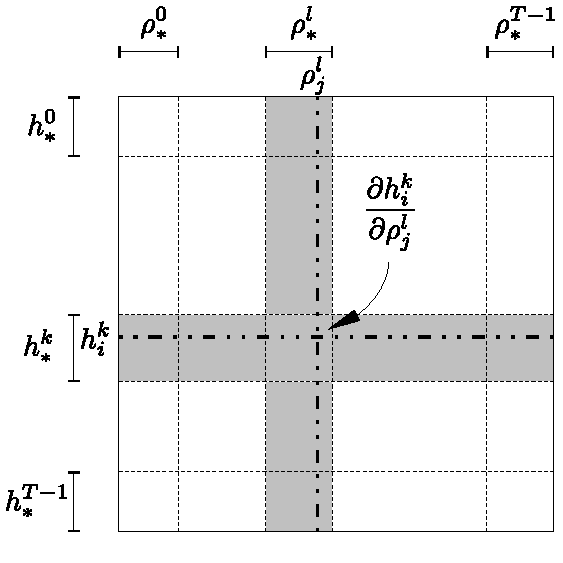
\includegraphics[width=0.45\columnwidth]{figs-gen/dstate}

}\texttt{\hfill{}}\subfloat[\label{fig:sparsity-diagram}Sparsity structure of the $\Hx$ matrix.
Besides the diagonal blocks, which are identity matrices, blocks where
$l\neq\tind-1$ are zero.]{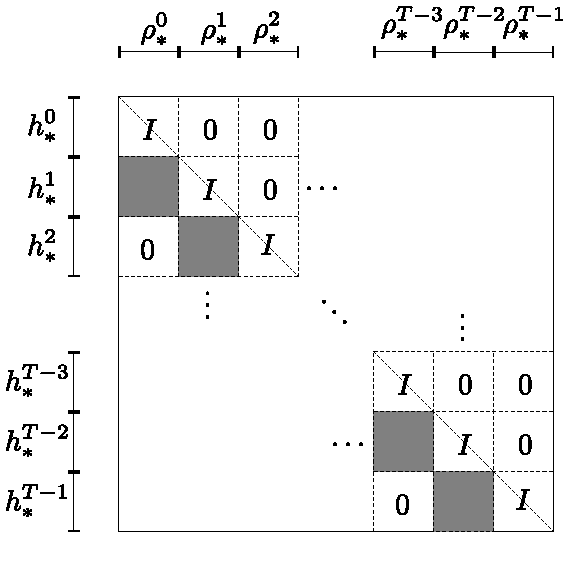
\includegraphics[width=0.45\columnwidth]{figs-gen/sparsity-two}

\texttt{}

}

\caption{Structure of the $\Hx$ matrix.}


\end{figure}
Similarly for $\Hu$, we take a control parameter $\condiscrete jl\in\control$,
and derive the expression:

\begin{align}
\pfrac{\syseq_{\link}^{\tind}}{\condiscrete jl}= & +\frac{\Delta t}{L_{i}}f'\left(\RS_{\jdown{\link}}\left(\juncstate{\jdown{\link}}{\tind-1},\junccon{\jdown{\link}}{\tind-1}\right)_{\link}\right)\pfrac{}{\condiscrete jl}\left(\RS_{\jdown{\link}}\left(\juncstate{\jdown{\link}}{\tind-1},\junccon{\jdown{\link}}{\tind-1}\right)_{\link}\right)\label{eq:dhdvfull} \\
& -\frac{\Delta t}{L_{i}}f'\left(\RS_{\jup{\link}}\left(\juncstate{\jup{\link}}{\tind-1},\junccon{\jup{\link}}{\tind-1}\right)_{\link}\right)\pfrac{}{\condiscrete jl}\left(\RS_{\jup{\link}}\left(\juncstate{\jup{\link}}{\tind-1},\junccon{\jup{\link}}{\tind-1}\right)_{\link}\right)\nonumber                       
\end{align}
or for the composed Godunov junction flux solver $\god_{\jn}$:

\begin{equation}
\pfrac{\syseq_{\link}^{\tind}}{\condiscrete jl}=\frac{\Delta t}{L_{i}}\left(\pfrac{}{\condiscrete jl}\left(\god_{\jdown{\link}}\left(\juncstate{\jdown{\link}}{\tind-1},\junccon{\jdown{\link}}{\tind-1}\right)\right)_{\link}-\pfrac{}{\condiscrete jl}\left(\god_{\jup{\link}}\left(\juncstate{\jup{\link}}{\tind-1},\junccon{\jup{\link}}{\tind-1}\right)\right)_{\link}\right)\label{eqdhdvgod}.
\end{equation}


Analyzing~\eqref{eq:dhdufull}, the only partial terms that are not
trivial to compute are $\pfrac{}{\discrete jl}\left(\RS_{\jdown{\link}}\left(\juncstate{\jdown{\link}}{\tind-1},\junccon{\jdown{\link}}{\tind-1}\right)_{\link}\right)$
and $\pfrac{}{\discrete jl}\left(\RS_{\jup{\link}}\left(\juncstate{\jup{\link}}{\tind-1},\junccon{\jup{\link}}{\tind-1}\right)_{\link}\right)$.
Similarly for~\eqref{eq:dhdvfull}, the only nontrivial terms are
$\pfrac{}{\condiscrete jl}\left(\RS_{\jdown{\link}}\left(\juncstate{\jdown{\link}}{\tind-1},\junccon{\jdown{\link}}{\tind-1}\right)_{\link}\right)$
and $\pfrac{}{\condiscrete jl}\left(\RS_{\jup{\link}}\left(\juncstate{\jup{\link}}{\tind-1},\junccon{\jup{\link}}{\tind-1}\right)_{\link}\right)$.
Once one obtains the solutions to these partial terms, then one can
construct the full $\Hx$ and $\Hu$ matrices and use~\eqref{eq:adjoint}
and~\eqref{eq:adjoint-grad} to obtain the gradient value.

As these expressions are written for a general scalar conservation
law, the only steps in computing the gradient that are specific to
a particular conservation law and Riemann solver are computing the
derivative of the flux function $f$ and the partial derivative terms
just discussed. These expressions are explicitly calculated for the
problem of optimal ramp metering in Section~(\ref{sec:Applications-to-Optimal}).


\subsection{Complexity of Solving Gradient via Forward Method vs. Adjoint Method\label{sub:Complexity-of-solving}}

This section demonstrates the following proposition:

\begin{prop}
\textup{The total complexity for the adjoint method on a scalar hyperbolic
network of PDEs is }$O(\ntime\left(\degree{\state}\nlinks+\degree{\control}\ncontrols\right))$.\end{prop}

We can show the lower-triangular structure and invertibility of $\Hx$
by examining~\eqref{eq:init-ge} and~\eqref{eq:main-ge}. For $\tind\in\intrange 1{\ntime-1}$,
we have that $\syseq_{\link}^{\tind}$ is only a function of $\discrete{\link}{\tind}$
and of the state variables from the previous time-step $\tind-1$.
Thus, based on our ordering scheme in Section~\ref{sec:State,-control,-and}
of ordering variables by increasing time-step and ordering constraints
by corresponding variable, we know that the diagonal terms of $\Hx$ are
always $1$ and all upper-triangular terms must be zero (since those
terms correspond to constraints with a dependence of \emph{future}
values). These two conditions demonstrate both that $\Hx$ is lower-triangular
and is invertible due to the ones along the diagonal.

Additionally, if we consider taking partial derivatives with respect
to the variable $\discrete jl$, then we can deduce from Equation~\eqref{eq:main-ge}
that all partial terms will be zero except for the diagonal term,
and those terms involving constraints at time $j+1$ with links connecting
to the downstream and upstream junctions $\jdown j$ and $\jup j$
respectively. To summarize, $\Hx$ matrices for systems described
in Section~\ref{sec:State,-control,-and} will be square, invertible,
lower-triangular and each column will have a maximum cardinality equal
to $\degree{\state}$ in~\eqref{eq:dx}. The sparsity structure of
$\Hx$ is depicted in Fig.~\ref{fig:sparsity-diagram}.

Using the same line of argument for the maximum cardinality of $\Hx$,
we can bound the maximum cardinality of each column of $\Hu$. Taking
a single control variable $\condiscrete jl$, the variable can only
appear in the constraints at time-step $j+1$ that correspond to a link
that connects to a junction $\jn$ such that $\condiscrete jl\in\junccon{\jn}{l+1}$.
These conditions give us the expression for $\degree{\control}$ in~\eqref{eq:dv},
or the maximum cardinality over all columns in $\Hu$.

If we only consider the lower triangular form of $\Hx$, then the
complexity of solving for the gradient using the forward system is
$O(\left(\nlinks\ntime\right)^{2}\ncontrols\ntime)$, where the dominating
term comes from solving~\eqref{eq:j-v}, which requires the solution
of $\ncontrols\ntime$ separate $\nlinks\ntime\times\nlinks\ntime$
lower-triangular systems. The lower-triangular system allows for forward
substitution, which can be solved in $O(\left(\nlinks\ntime\right)^{2})$
steps, giving the overall complexity $O(\left(\nlinks\ntime\right)^{2}\ncontrols\ntime)$.
The complexity of computing the gradient via the adjoint method is
$O(\left(\nlinks\ntime\right)^{2}+\left(\nlinks\ntime\right)\left(\ncontrols\ntime\right))$,
which is certainly more efficient than the forward-method, as long
as $\ncontrols\ntime>1$. The efficiency is gained by considering
that~\eqref{eq:adjoint} only requires the solution of a single $\nlinks\ntime\times\nlinks\ntime$
\emph{upper}-triangular system (via backward-substitution), followed
by the multiplication of $\lambda^{T}H_{v}$, an $\nlinks\ntime\times\nlinks\ntime$
and an $\nlinks\ntime\times\ncontrols\ntime$ matrix in~\eqref{eq:adjoint-grad},
with a complexity of $O(\left(\nlinks\ntime\right)^{2}+\left(\nlinks\ntime\right)\left(\ncontrols\ntime\right))$.

For the adjoint method, this complexity can be improved upon by considering
the sparsity of the $\Hx$ and $\Hu$ matrices, as detailed in Section~\ref{sub:Complexity-of-solving}.
For the backward-substitution step, each entry in the $\lambda$ vector
is solved by \emph{at most} $\degree{\state}$ multiplications, and
thus the complexity of solving~\eqref{eq:adjoint} is reduced to
$O(\degree{\state}\nlinks\ntime)$. Similarly, for the matrix multiplication
of $\lambda^{T}H_{v}$, while $\lambda$ is not necessarily sparse,
we know that each entry in the resulting vector requires at most $\degree{\control}$
multiplications, giving a complexity of $O(\degree{\control}\ncontrols\ntime)$. Furthermore, if a sparse implementation of the $\Hx$ and $\Hu$ matrices are used, then memory usage will also scale linearly with the number of state and control variables.

\section{Decentralized Control of Flow Networks}
\label{sec:admm-intro}

Finite-horizon optimal control is a popular method for computing predictive control strategies for dynamical systems~\cite{Reilly2013AdjointBased,Bayen2006AdjointBased,Raffard2008AdjointBased}, its applicability growing with the increase of computational power and pervasiveness of physical sensing. In general, a finite-horizon optimal control problem will take the following form:

\begin{align}
	\label{eq:fhop}
	\min_{x\in X} & \quad f\left(s, x\right) \\
	\text{subject to:} & \quad s = g\left(x\right)
\end{align}

where $x$ represents the vector of control variables belonging to the set of feasible controls $X$ (which we may assume to be $\Re^n$ for simplicity), $s$ represents the vector of ``state'' variables, constrained to be a deterministic function $g\left(x\right)$ of the control, and $f$ is some objective function of the control and state we wish to minimize.

\paragraph*{Related Work in Distributed Optimization}
Much attention has recently been given to distributed methods for finite-horizon optimal control problems, where $g$ is assumed to be linear and $f$ is assumed to be quadratic or convex. Distributed optimization has been found useful for at least two reasons. Firstly, the parallelizability of the individual sub-problems allows for faster computation time and better overall convergence properties~\cite{Donoghue2013Splitting,Frejo2011Feasible,Pu2014Fast,Giselsson2013Accelerated}. Secondly, physical systems often have their controls physically distributed in space, creating a need for distributed control algorithms which limit the amount of shared information and communication between subsystems~\cite{Venkat2008Distributed,mota2012distributed,camponogara2009distributed}.

Different assumptions on the structure, smoothness, and convexity of $f$, $X$ and $g$ leads to different convergence bounds and communication bounds in distributed optimization. A method for decoupling the quadratic terms from the nonquadratic terms in optimal control, presented in~\cite{Donoghue2013Splitting} leads to efficient caching techniques shown to be effective in FPGA applications. A distributed gradient descent-based approach is given in~\cite{camponogara2009distributed}, which has $O\left(\frac{1}{\sqrt{k}}\right)$ convergence to the global optimum in the general case, where $k$ is the number of iterations of the algorithm.  A common dual-decomposition technique employed for distributed optimal control is the \emph{alternating directions method of multipliers}~\cite{Boyd2010Distributed,Donoghue2013Splitting,gabay1976dual} (ADMM), which has been shown to have $O\left(\frac{1}{k}\right)$ convergence under certain assumptions of the smoothness and decomposability of the objectives~\cite{Wei2013On}. Additionally, an accelerated version of ADMM, based on Nesterov's algorithm~\cite{Nesterov1983Method} can give $O\left(\frac{1}{k^2}\right)$ convergence when the decomposed objectives are smooth~\cite{Pu2014Fast}.

When the coupling between systems takes on some sparse form, then one can devise algorithms with limited communication, which can be beneficial from a latency and  architectural standpoint. Optimal control problems where subsystems have disjoint state variables but coupled control variables have been shown to be amenable to decomposition techniques for distributed optimization~\cite{Giselsson2013Accelerated,camponogara2009distributed}, where~\cite{mota2012distributed} shows how ADMM decomposition leads to less communication without a decrease in solution accuracy.

In~\cite{Giselsson2013Accelerated,mota2012distributed,camponogara2009distributed}, the subsystems with disjoint state are modeled as agents tasked with optimizing over their own subsystem, where agents which share some control variables are connected by some edge in a communication graph. Thus, the more sparse the coupling of systems, the lesser the communication requirements. Such a model is referred to as \emph{multi-agent optimization}~\cite{Wei2013On}. In systems with coupling due to physical proximity, this consequence has the added benefit of requiring only physically local communication, and removes the need for any centralized controller or hub for communication. In~\cite{Wei2013On}, an asynchronous form of ADMM (subsequently referred to as A-ADMM) is presented for multi-agent optimization, which permits agents to update themselves in arbitrary order, with communication only required between neighboring agents. The method in~\cite{Wei2013On} does not present an accelerated version and is shown to have $O\left(\frac{1}{k}\right)$ convergence.

\paragraph*{Subsystems with Coupled State}
One recurring assumption in the distributed optimization literature above is that subsystems have disjoint state variables. For network flow problems, where subsystems correspond to partitions of a network into subnetworks, such an assumption does not hold. To see this, one can imagine a traffic light timing plan causing a traffic jam which spreads across the entire freeway network~\cite{Reilly2013AdjointBased,Muralidharan2012Optimal} or a bottleneck of planes in an airspace affecting flight times throughout the air network~\cite{Bayen2006AdjointBased}. As a result, it is not possible to decompose the subsystems by only sharing control parameters without coupling each subsystem to all control variables and modeling the evolution of the entire network within each subsystem.

Yet, freeway traffic and air traffic subsystems have a very sparse coupling in their state variables. For instance, discrete traffic models~\cite{Monache2014PdeOde,daganzo1995cell} often assume that the speed of traffic on a particular section of road is only a function of the speed of traffic on neighboring links. Thus, each subnetwork subsystem would only share a small number of control variables and state variables with other subsystems, precisely those which physically share a border with the subsystem.

To exploit the sparsity of such systems, we develop a multi-agent optimization algorithm based on A-ADMM~\cite{Wei2013On} which permits each agent (subsystem) to share both control and state variables with neighboring agents, while still converging to the globally optimal control, given the standard assumption of convex objectives and linear constraints. At a high level, the algorithm ``relaxes'' the state variables \emph{external} to an agent while constraining \emph{internal} state variables to adhere to the subsystem's dynamics. Since A-ADMM eventually brings all shared variables between agents into \emph{consensus} (i.e. the difference between shared variables converges to zero), the relaxed external state variables will converge to satisfying the original constraints.

The rest of the section is structured as follows.
% Section~\ref{sec:admm-overview} gives an overview of ADMM and its application to consensus-type problems.
Section~\ref{sec:problem_statement} presents the general problem of posing a multi-agent optimal control problem, with the additional assumption that an agent may share both state and control variables with other agents. The problem is then posed in a form amenable to using the A-ADMM algorithm in Section~\ref{sec:algorithm}. A systematic approach to modeling an optimal control problem over a dynamical network as a multi-agent distributed optimization over subnetworks is given in Section~\ref{sec:distributed_optimization_of_coupled_dynamical_systems}, as well as a discussion on the suitability of the method for scaling model predictive control on dynamical networks. In Section~\ref{sec:minimizing_sub_objectives_using_the_adjoint_method}, we give an adjoint-based approach to solving the agent's subnetwork optimal control problem, suitable for applications with complex, non-convex dynamics. We then present the application of distributed, predictive ramp-metering control on freeway networks in Section~\ref{sec:ramp-metering-admm} followed by numerical results in Section~\ref{sec:numerical_results-admm} with comparisons to existing distributed approaches.
% We conclude with some final remarks in Section~\ref{sec:conclusion}.

\paragraph*{\textbf{Notation}}

For a vector $x$, let $x\left[i\right]$ be the $i$'th element of $x$, and similarly let $y\left[i,j\right]$ be the element of the two-dimensional vector in the $i$'th row and $j$'th column. If we have a vector $x$ with $card\left(x\right)=N$ and let $w$ be a subset of $ \{1,\ldots,N\}$, then let $x_w$ denote the vector selecting only those elements $x\left[i\right]$ where $i\in w$. If a vector $d$ is the concatenation $d = \left(a,b,c\right)$, then let $\left[d\right]_a$ be the sub-vector of $d$ corresponding to the original element $a$.

% \subsection{Distributed Optimization and ADMM}
% \label{sec:admm-overview}

% \todo{overview of admm and distributed optimization.}

\subsection{Optimization over Systems with Shared State}
\label{sec:problem_statement}

We wish to solve an optimization problem with a ``free'' global variable $x \in \Re^n$ and a ``dependent'' variable $s \in \Re^m$ which is a deterministic function of $x$.
We assume there is a partition of $s$ into $D$ disjoint subsets,
\[
s=\left(s_{u\left(1\right)},\ldots,s_{u\left(D\right)}\right),
\] where $u\left(i\right)$ are subsets of $ \{1,\ldots,m\} $.
The objective function is assumed to be the sum of $D$ sub-objectives, where sub-objective $f_i, i\in \{1,\ldots,D\} $ is a convex function of only variable $s_{u\left(i\right)}$~\footnote{We omit the dependency of the objective on the control variable in this presentation for simplicity. It is still easy in this form to add control variables into the objective by duplicating a control variable into the state.}.
Furthermore, $s_{u\left(i\right)}$ is assumed to be a function of some subset of $x$ and $s$.
Explicitly, for each $i\in {1,\ldots, D} $, there is well-defined, linear function $g_i$ and subsets $v\left(i\right)$ and $w\left(i\right)$ ($w\left(i\right) \cap u\left(i\right) = \emptyset$) where 
\[
s_{u\left(i\right)} = g_i\left(\left(x_{v\left(i\right)}, s_{w\left(i\right)}\right)\right).
\]
The tuple $\left(x_{v\left(i\right)}, s_{w\left(i\right)}\right)$ is the concatenation vector of $x_{v\left(i\right)}$ and $s_{w\left(i\right)}$.
We omit the double parenthesis in the rest, for simplicity. One can view $u\left(i\right), v\left(i\right), w\left(i\right), $ as the \emph{internal} state, the control, and the \emph{external} state, respectively, of group $i$. 
We can now express the optimization problem we wish to solve as:

\begin{align}
	\label{eq:problem-statement}
	\min_{x,s} & \quad \sum_{i = 1}^D f_i\left(s_{u\left(i\right)}\right) \\
	\text{subject to:} & \quad s_{u\left(i\right)} = g_i\left(x_{v\left(i\right)}, s_{w\left(i\right)}\right) \quad \forall i
\end{align}

Figure~\ref{sub:dep-graph-diagram} shows an example of how different sub-objectives may be coupled and Table~\ref{tab:dep-graph-subsets} summarizes how one constructs the $u\left(i\right), v\left(i\right), w\left(i\right)$ subsets from the state and control coupling.

\begin{figure}[t]
\centering
	\subfloat[Free and dependent variable coupling diagram.]{%
	\label{sub:dep-graph-diagram}%
	\includegraphics[width=.45\columnwidth]{previous-articles/admm/figures/dep-graph}
	}\\
	\subfloat[Summary of resultant state, control, and external state subsets.]{%
    \begin{tabular}{|l|c|c|c|}
    \hline
    Group $i$ & $u\left(i\right)$ & $v\left(i\right)$ & $w\left(i\right)$\\ \hline
    $i=1$ & \{1,2\}       & \{1\}        & \{\}        \\ \hline
    $i=2$ & \{3\}        & \{1,2\}       & \{4,5\}       \\ \hline
    $i=3$ & \{4,5\}        & \{3\}       & \{3\}       \\ \hline
    \end{tabular}\label{tab:dep-graph-subsets}}\hfill%
    \subfloat[Summary of shared control and state between groups]{
    \begin{tabular}{|l|c|c|c|}
    \hline
    Edge $\left(i,j\right)$ & $v\left(i\right) \cap v\left(j\right)$ & $u\left(i\right) \cap w\left(j\right)$ & w$\left(i\right) \cap u\left(j\right)$  \\ \hline
    $i,j=1,2$ & \{1\}       & \{\}        & \{\}        \\ \hline
    $i,j=2,3$ & \{\}        & \{3\}       & \{4,5\}       \\ \hline
    $i,j=1,3$ & \{\}        & \{\}       & \{\}       \\ \hline
    \end{tabular}
\label{tab:dep-graph-edges}
}
    \caption{Example of optimization problem partitioned into $D=3$ disjoint state variable groups with shared control and external state variables. Figure~\ref{sub:dep-graph-diagram} shows the partitioned problem, where an arrow depicts a dependency of a partition group on an external state variable or control variable. The arrows allow us to compute the $u\left(i\right), v\left(i\right), w\left(i\right)$ subsets for each group $i$, which is summarized in Table~\ref{tab:dep-graph-subsets}. The dependency graph $(V,E)$ is computed using the subsets in Table~\ref{tab:dep-graph-subsets}, which is summarized in Table~\ref{tab:dep-graph-edges} and reveals that edges exist for groups $\left(1,2\right)$ and $\left(2,3\right)$, but not for $\left(1,3\right)$.}%
    \label{fig:dep-graph}
  \end{figure}


\paragraph*{Dependency Graph}

There are no assumptions on the subsets $v\left(i\right)$ and $w\left(i\right)$, which implies that the value of each sub-objective $f_i$ is coupled to not just the sub-vector $s_{u\left(i\right)}$, but also the global variable $x$, and other sub-vectors $s_{u\left(j\right)}$. We can express this coupling as a dependency graph $\left(V,E\right)$, where vertices $V$ are each sub-problem $i\in \{1,\ldots, D\} $ and an edge $\left(i,j\right)\in E$ exists whenever

\begin{enumerate}
	\item  $w\left(i\right) \cap u\left(j\right) \neq \emptyset$ ($g_i$ is a function of some variable in $s_{u\left(j\right)}$), \textbf{or}
	\item $v\left(i\right) \cap v\left(j\right) \neq \emptyset$ (there is some $x\left[k\right]$ which both $g_i$ and $g_j$ depend upon).
\end{enumerate}
 
Let the neighboring edges of node $i\in V$ be denoted by $E\left(i\right)$. A dependency graph construction for the example in Figure~\ref{sub:dep-graph-diagram} is summarized in Table~\ref{tab:dep-graph-edges}.

In Section~\ref{sec:algorithm}, we devise a distributed algorithm solve Problem~\eqref{eq:problem-statement} with the following requirements:

\begin{enumerate}
	\item Each processing node corresponds to a sub-objective node in the dependency graph.
	\item Each node can be updated in parallel.
	\item Each node $i$ only exchanges information with its neighbors $E\left(i\right)$ in the dependency graph $\left(V,E\right)$.
	\item The algorithm is asynchronous and decentralized, i.e. no central process is required and nodes can be updated arbitrarily.
\end{enumerate}

% \subsection{Asynchronous ADMM and Subnetwork Splitting}
% \label{sec:algorithm}

% section problem_statement (end)

\subsection{Asynchronous-ADMM Algorithm} % (fold)
\label{sec:algorithm}

We now reformulate Problem~\eqref{eq:problem-statement} to permit a distributed solution method via A-ADMM.  For each node $i\in V$, we replicate the ``shared variables'' $x_{v\left(i\right)}$ and $s_{w\left(i\right)}$ as $\bar{x}_i$ and $\bar{s}_i$ respectively, and reformulate Problem~\eqref{eq:problem-statement} as:

\begin{align}
	\label{eq:replicate-problem-statement}
	\min_{x} & \quad \sum_{i = 1}^D f_i\left(s_{u\left(i\right)}\right) \\
	\text{subject to:} & \quad s_{u\left(i\right)} = g_i\left(\bar{x}_i, \bar{s}_i\right) \quad \forall i  \label{eqn:state-constraint-decoupled} \\
	 & \quad \bar{s}_i = s_{w\left(i\right)} \quad \forall i \label{eqn:state-consensus} \\
	 & \quad \bar{x}_i = x_{v\left(i\right)} \quad \forall i \label{eqn:control-consensus} 
\end{align}

The variable replication allows Constraint~\eqref{eqn:state-constraint-decoupled} in Problem~\eqref{eq:replicate-problem-statement} to be decoupled across nodes. To decouple Constraints~\eqref{eqn:state-consensus} and~\eqref{eqn:control-consensus}, we follow a modified process from~\cite{Wei2013On}.

First, we replicate each subset $s_{u\left(i\right)}$ with a vector $s_i$ local to node $i \in V$, and then concatenate all local variables into a single variable $y_i = \left(s_i, \bar{x}_i, \bar{s}_i\right)$, such that $y_i$ is restricted to the space:
\[
Y_i = \{\left(s_i,\bar{x}_i, \bar{s}_i\right) : s_i = g_i\left(\bar{x}_i, \bar{s}_i\right)\}.
\]
Finally, we can repose Constraints 2 and 3 in an \emph{edge-wise} fashion as follows. For each edge $e = \left(i,j\right) \in E$, let $y_{i,e}$ and $y_{j,e}$ be the sub-vectors of $y_i$ and $y_j$ that are coupled through $g_j$ and $g_i$, respectively. Then Problem~\eqref{eq:problem-statement} becomes:

\begin{align}
	\label{eq:edge-problem-statement}
	\min_{(y_i \in Y_i)_{i \in V}} & \sum_{i = 1}^D f_i\left(\left[y_i\right]_{s}\right) \\
	\text{subject to:} & \quad y_{i,e} = y_{j,e} \quad \forall e\in E
\end{align}

By moving the edge constraints into the objective through a standard Lagrange multiplier approach, and adding a regularization term which is equal to zero for feasible solutions~\cite{Boyd2010Distributed}, we can construct the augmented Lagrangian $\mathcal{L}$ formulation (with tunable augmenting coefficient $\augterm$), and express the optimization problem as:

\begin{align}
	\label{eq:lagrangian}
	\min_{y = (y_i)_{i \in V}} \max_{\lambda = \left(\lambda_e\right)_{e \in E}} & \mathcal{L} \left(y,\lambda\right) :=  \\
	& \sum_{i = 1}^D f_i\left(\left[y_i\right]_{s}\right) + \\
	& \sum_{e\in E} \lambda_e^T \left(y_{i,e} - y_{j,e}\right) + \augterm \|y_{i,e} - y_{j,e}\|_2^2, \nonumber
\end{align}
	
The above form permits us to apply the A-ADMM algorithm as proposed and analyzed in~\cite{Wei2013On}, and shown in Algorithm~\ref{alg:a-admm}. At a high-level, the algorithm iterates by first randomly selecting an edge $e = \left(i,j\right)$ from $E$. Then, nodes $i$ and $j$ update $y_i$ and $y_j$ respectively by minimizing the Lagrangian in Equation~\eqref{eq:lagrangian} in parallel, while holding all other variables $\{\lambda_e'\}_{e' \neq e}, \{y_k\}_{i\notin \{i,j\}}$ constant. The new $y_i$ and $y_j$ values are used to update the dual $\lambda_e$ variables by applying a dual-ascent method~\cite{Boyd2010Distributed}. Finally, the process is repeated \emph{ad-infinitum} by updating a new edge selected from $E$, until some convergence or termination criteria are reached.

Section~\ref{sec:minimizing_sub_objectives_using_the_adjoint_method} presents an efficient solution method, based on discrete adjoint computations, to solving the subproblem on Line 4 of Algorithm~\ref{alg:a-admm}.

\begin{remark} The equation in Line~\ref{lst:local-state-update} differs slightly from the augmented Lagrangian in Equation~\eqref{eq:lagrangian} and is the result of a number of algebraic manipulations, which are explicitly derived in~\cite{Boyd2010Distributed,Wei2013On}.
\end{remark}
\begin{remark}
We introduce the asymmetric coefficient $\Lambda_{q,e}$ to account for the fact that the terms for edge $e\in E\left(q\right)$ in Line~\ref{lst:local-state-update} depend upon whether the updating problem $q$ was the first or second term ($i$ or $j$) in the edge pair.
\end{remark}

\begin{algorithm}[t]  % enter the algorithm environment
\caption{Asynchronous Edge Based ADMM} % give the algorithm a caption
\label{alg:a-admm}       % and a label for \ref{} commands later in the document
\begin{algorithmic}[1]% enter the algorithmic environment
    \WHILE{Not Converged}
    \STATE Select edge $\left(i,j\right) \in E$
        \FOR{$q \in \left(i,j\right)$}
        \STATE $ y^{k+1}_q \gets \arg \min_{y \in Y_q} f_q\left(\left[y\right]_{s}\right) - \sum_{e \in E\left(q\right)}
        \Lambda_{q,e} \lambda^{k,T}_{e} \left(y_{q,e} - \bar{y}^{k}_{e} \right) +
        \frac{\augterm}{2} \|y_{q,e} - \bar{y}^{k}_{e}\|_2^2 $ \label{lst:local-state-update}
        \ENDFOR
        \STATE $\lambda^{k+1}_{e} \gets \lambda^{k+1}_{e} - \frac{\augterm}{2} \left(y^{k+1}_{i,e} - y^{k+1}_{j,e}\right)$
        \FOR{$q \notin \left(i,j\right)$}
        \STATE $a^{k+1} \gets a^{k}$
        \ENDFOR
    \ENDWHILE
    \STATE Note: $\tilde{y}^{k}_{e} = \frac{1}{2} \left(y^k_{i,e} + y^k_{j,e}\right)$
    \STATE Note: $\Lambda_{q,e} = \begin{cases} 1 & \quad q = i \\ -1 & \quad q = j \end{cases} \quad e = (i,j)$
\end{algorithmic}
\end{algorithm}

% section minimizing_sub_objectives_using_the_adjoint_method (end)

\subsection{Distributed Optimization on Coupled Dynamical Systems} % (fold)
\label{sec:distributed_optimization_of_coupled_dynamical_systems}

Physical transport systems, such as freeway traffic networks~\cite{Reilly2013AdjointBased,daganzo1995cell} or gas pipelines~\cite{Gugat2011Gas} are often naturally expressed as a network of individual dynamical systems which influence one another at contact points, or \emph{junction points}. Given the coupling in dynamics across the entire network, optimizing over partitioned sub-systems, with no communication between systems, will lead to \emph{greedy} solutions over the individual systems and sub-optimal global results~\cite{Ramon2013}. Thus, any distributed, globally optimal control scheme applied to such systems must account for the \emph{shared state} between the systems. We now show how this can be done using the multi-agent A-ADMM approach. Furthermore, we show how the algorithm naturally leads to a communication scheme which mirrors the physical structure of the underlying physical network.

Assume have some discrete-time, discrete-space dynamical system which possesses some network-like dynamical coupling in space. Specifically, consider a graph $\left(V^d, E^d\right)$ (not to be confused with the dependency graph $\left(V,D\right)$ in Section~\ref{sec:problem_statement}, where the $d$ superscript is added to denote the \emph{dynamical} network) where $E^d$ represent the discrete-space \emph{cells} and $V^d$ are the \emph{junction points} where cells connect to one another, i.e. each cell in $E^d$ has a corresponding upstream and downstream junction both in $V^d$.  Each discrete space ``cell'' $c \in \{1,\ldots,N_d\} $ has for each discrete time step $k \in \{1,\ldots,T_d\} $ both a control variable $x\left[c,k\right] \in \Re$ and a state variable $s\left[c,k\right] \in \Re$. The variable $s\left[c,k\right]$ is assumed to be a function of all state and control variables that satisfy two conditions:

\begin{itemize}
	\item the time-step is $k-1$, and
	\item the cell must share a junction with cell $c$.
\end{itemize}

Next, we wish to express a distributed optimization problem subject to the above dynamics in the form of Problem~\eqref{eq:problem-statement}. To do so, we assume a partition of $\left(V^d,E^d\right)$ into $D$ \emph{sub-networks}, which implies a partition of $E^d$ into $D$ subsets $\left(E^d_1,\ldots, E^d_D\right)$ and assume an objective $f$ which is splittable across the state variables internal to each sub-network. This leads to a state partitioning $s=\left(s_{u\left(1\right)}, \ldots, s_{u\left(D\right)}\right)$, where $ \left(c,k\right) \in u\left(i\right)$ iff $c \in E^d_i$.

Based on the two conditions for state dependencies above, we can deduce that the state of a sub-network depends on the control and state both internal to the sub-network and directly \emph{neighboring} the sub-network. Explicitly, for sub-network $i$, we can express the dependent control variables as $x_{v\left(i\right)}$ where $\left(c,k\right)\in v\left(i\right)$ iff $c \in E^d_i$ or $c$ neighbors a cell in $E^d_i$. Similarly, the shared state for sub-network $i$ is $s_{w\left(i\right)}$, where $\left(c,k\right)\in w\left(i\right)$ iff $c \notin E^d_i$ and $c$ neighbors a cell in $E^d_i$. Finally, we conclude that there exists some update equation $g_i$, specific to the particular dynamical system, where the constraint on $s_{u\left(i\right)}$ can be expressed familiarly as $s_{u\left(i\right)} = g_i\left(x_{v\left(i\right)}, s_{w\left(i\right)}\right)$.

\begin{figure}
	\subfloat[Complete network]{
	\includegraphics[width=.4\columnwidth]{previous-articles/admm/figures/net-1}
	\label{subfig:net-1}
	} \hfill
	\subfloat[Solid subnetwork with two shared links]{
	\includegraphics[width=.4\columnwidth]{previous-articles/admm/figures/net-2}
	\label{subfig:net-2}
	}\\
	\subfloat[Dotted subnetwork with three shared links]{
	\includegraphics[width=.4\columnwidth]{previous-articles/admm/figures/net-3}
	\label{subfig:net-3}	
	} \hfill
	\subfloat[Dash-dotted subnetwork with three shared links]{
	\includegraphics[width=.4\columnwidth]{previous-articles/admm/figures/net-4}
	\label{subfig:net-4}	
	}
	\label{fig:net-example}
	\caption{A network is partitioned into three subnetworks: solid, dashed, and dash-dotted. Each subnetwork will share state with neighboring subnetworks. For a subnetwork $i$, the cells neighboring $i$, denoted by $E^d_i$, are shown in black, while those excluded from $E^d_i$ are shown in gray.}
\end{figure}

As an example, we can consider the network in Figure~\ref{subfig:net-1}, which is partitioned into three subnetworks based on line-style. We see that four of the edges share a single junction between the three subnetworks. Thus, the dynamics assumed above implies that each subnetwork will share state with each other subnetwork. Specifically, the solid-lined network in Figure~\ref{subfig:net-2} shares one cell each from the other two subnetworks, while the dashed and dash-dotted subnetworks in Figures~\ref{subfig:net-3} and~\ref{subfig:net-4} share two cells with the solid subnetwork and one cell with the opposite subnetwork. It's worth reiterating that while each optimizing agent may have different values of the state on a particular cell in the network during intermediate stages of the A-ADMM algorithm, each copy of the state will eventually come into consensus as the shared-state A-ADMM algorithm converges.

\paragraph*{Local Communication Requirements}

At this point, all relevant parameters to Problem~\eqref{eq:problem-statement} have been specified. The assumption on the dynamical network coupling leads to a desirable dependency graph $\left(V,E\right)$ for the system above. Since each sub-network only requires shared state from neighboring sub-networks in the sense of the \emph{physical} network $\left(V^d,E^d\right)$, then the dependency graph $\left(V,E\right)$ is constructed by assigning a sub-network to each node $V$ and adding an edge $\left(i,j\right)$ to $E$ only for those sub-networks $i$ and $j$ which physically neighbor each other. 

Thus, the A-ADMM algorithm guarantees that communication only take place between physically neighboring systems. This is useful for situations where there are limitations in the networking capabilities due to physical distance, such as freeway traffic control systems, where collaborations may only exist for those districts near each other.

Furthermore, the formulation allows for a completely decentralized and asynchronous implementation of the global optimization problem. If, for instance, all nodes are managed by independent agencies with varying computational limits, then there are several practical benefits to the approach. For a single sub-network, since only information that is directly adjacent to other sub-networks needs to be shared with other sub-networks, much of the internal formulation of the sub-network can be made completely hidden from the larger network. The asynchronicity of the algorithm also permits for neighboring agencies to exchange information in an ad-hoc manner, and not be bottlenecked by slower updates between separate sub-networks.

\paragraph*{Scalability of Subnetwork Splitting for Model Predictive Control}

A common application of finite-horizon optimal control is in the context of model predictive control (MPC)~\cite{Reilly2013AdjointBased,Frejo2011Feasible}, where optimal control policies are recomputed in a \emph{rolling-horizon} fashion. Given the optimal control problem beginning at a time-step $t$,
 
\begin{align}
	\label{eq:fhop-mpc}
	\min_{x = \{x_t,\ldots, x_{t + T}\}} & \quad f_t^{t + T}\left(s, x\right) \\
	\text{subject to:} & \quad s = g_t^{t + T}\left(x\right) \nonumber,
\end{align}

MPC chooses the control policy $x_t$ to apply at time-step $t$ by solving for $x = \{x_t,\ldots, x_{t + T}\}$ in Equation~\eqref{eq:fhop-mpc} using a prediction horizon of $T$ and updating the objective $f_t^{t+T}$ and constraints $g_{t}^{t + T}$ based on the latest estimates of the initial conditions and boundary conditions.

In applications such as freeway onramp metering, a limiting factor in choosing an optimization time-horizon is the accuracy of the predictions of the boundary conditions, or specifically, anticipating future vehicle demands on freeway onramps. At some point, increasing the time-horizon will only decrease the effectiveness of the control due to the deviation in predicted model state versus reality. Thus, it is often practical to consider the time-horizon fixed in MPC applications, at which point the scalability with respect to network size becomes of importance.

For freeway networks with very small branching factors, it is reasonable to assume the following:

\begin{itemize}
	\item For each subnetwork, the number of bordering links is \emph{constant}.
	\item The number of shared state and control variables grows \emph{linearly} with the time-horizon for each subnetwork.
	\item The number of subnetworks scales linearly with network size (for fixed-size subsystems).
\end{itemize}

 One concludes that the amount of communication required for the A-ADMM subnetwork splitting method would scale linearly with the network size and quadratically with time-horizon length. If we were to instead decompose our system, for instance, across time-slices, the communication requirement would scale quadratically with network size and linearly with time-horizon length. Given our assumption of a fixed time-horizon, the subnetwork splitting approach for network-flow MPC has the added benefit of better scaling in the communication requirements.

\subsection{Solving Sub-problems via the Adjoint Method} % (fold)
\label{sec:minimizing_sub_objectives_using_the_adjoint_method}

What is not explicitly expressed in Algorithm~\ref{alg:a-admm} is a solution method for Step~\ref{lst:local-state-update}:

\begin{align}
	\label{eq:sub-op-problem}
	y^{k+1}_i & = \arg \min_{y \in Y_i}
        f_i\left(\left[y\right]_{s}\right) - \\
        & \sum_{e \in E\left(i\right)}
        \Lambda_{i,e} \lambda^{k,T}_{e} \left(y_{i,e} - \bar{y}^{k}_{e} \right) +
        \frac{\augterm}{2} \|y_{i,e} - \bar{y}^{k}_{e}\|_2^2 \nonumber
\end{align}
In the more general case of non-convex update equations $g_i$ and objectives $f_i$, it is difficult to find even local optima for $y_i$ over the space $Y_i$ using gradient-descent methods: a result of the difficulty of projecting and expensiveness of computing gradients in $Y_i$.

Since $\left[y_i\right]_{s}$ is a deterministic function of the unconstrained variables $\left[y_i\right]_{\bar{x}}$ and $\left[y_i\right]_{\bar{s}}$, it becomes more efficient to eliminate $\left[y_i\right]_{s}$ from the search space and concatenate $\left[y_i\right]_{\bar{x}}$ and $\left[y_i\right]_{\bar{s}}$ into a single ``free'' variable $\bar{r}_i := \left(\left[y_i\right]_{\bar{x}},\left[y_i\right]_{\bar{s}} \right)$. Similar to the convention for $y_{i,e}$ and $y_{j,e}$, we denote $\left(\bar{r}_{i,e}, \bar{r}_{j,e}\right)$ and $\left(\bar{s}_{i,e}, \bar{s}_{j,e}\right)$ as the free variables and constrained state variables, respectively, shared between nodes $i$ and $j$. Then we can repose the sub-optimization Problem~\eqref{eq:sub-op-problem} in the following way. We let

\begin{align*}
\bar{f_i}\left(s_i,\bar{r}_i\right) := & f_i\left(\left[y\right]_{s}\right) - \\
        & \sum_{e \in E\left(i\right)}
        \Lambda_{i,e} \lambda^{k,T}_{e} \left(r_{i,e} - \bar{r}^{k}_{e} \right) +
        \frac{\augterm}{2} \|r_{i,e} - \bar{r}^{k}_{e}\|_2^2 + \\
        & \sum_{e \in E\left(i\right)}
        \Lambda_{i,e} \lambda^{k,T}_{e} \left(s_{i,e} - \bar{s}^{k}_{e} \right) +
        \frac{\augterm}{2} \|s_{i,e} - \bar{s}^{k}_{e}\|_2^2        
\end{align*}
be the ``augmented'' sub-objective accounting for the additional ADMM terms for subproblem $i$, where $\bar{r}_e,\bar{s}_e$ denotes the vector mean of $r_{i,e},r_{j,e}$ and $s_{i,e},s_{j,e}$ respectively. Also, if we let the concatenated subsystem equations be:

\[
H_i\left(s,r\right) :=s - g_i\left(\left[r\right]_{\bar{x}}, \left[r\right]_{\bar{s}} \right),
\]

then we have

\begin{align}
	\label{eq:sub-op-simple}
	\left(s^{k+1}_i, \bar{r}^{k+1}_i\right) & = \arg \min_{s,r} \bar{f}_i\left(s, r\right) \\ 
	\text{subject to:} & \quad H_i\left(s,r\right) = 0
\end{align}

The form of Problem~\eqref{eq:sub-op-simple} permits us to apply the \emph{discrete adjoint method} (Section~\ref{sec:discrete-adjoint-method}) to compute gradients of $\bar{f}_i$ at some search point $\bar{r}^0_i$. If we let $s^0_i$ be defined so that $H_i\left(s^0_i,\bar{r}_i^0\right) = 0$, then we arrive at the following expression for the gradient:

\begin{align}
	\label{eq:adjoint-grad-admm} \nabla_{r} \bar{f}_i\left(s^0_i,\bar{r}_i^0\right)  =  \gamma^T \frac{\partial H_i\left(s^0_i,\bar{r}_i^0\right)}{\partial r} & + \frac{\partial \bar{f}_i\left(s^0_i,\bar{r}_i^0\right)}{\partial r} \\ \text{subject to: } \quad \frac{\partial H_i\left(s^0_i,\bar{r}_i^0\right)}{\partial s}^T \gamma & = -\frac{\partial \bar{f}_i\left(s^0_i,\bar{r}_i^0\right)}{\partial s}^T, \label{eq:adjoint-system}
\end{align}

where $\gamma$ is the \emph{discrete adjoint} variable and Equation~\eqref{eq:adjoint-system} is the \emph{discrete adjoint} system.

\subsection{Applications to Asynchronous, Decentralized Ramp Metering}
\label{sec:ramp-metering-admm}

We apply distributed optimization via subnetwork splitting to the problem of coordinated, predictive freeway onramp metering~\cite{Papageorgiou1991Alinea,Frejo2011Feasible,Reilly2013AdjointBased}, where traffic lights on freeway onramps are used to regulate the flow entering freeway mainlines in order to prevent congestion and improve such metrics as driver travel time and speed variability. The term \emph{coordinated} indicates that many traffic lights along a freeway stretch will act cooperatively, given that conditions near one onramp may eventually affect conditions at a neighboring onramp. The term \emph{predictive} indicates that the metering strategy should anticipate future conditions on the roadway using traffic demand predictions and an underlying model of the evolution of the freeway system.

Following the discretized freeway model in~\cite{Monache2014PdeOde,Reilly2013AdjointBased}, the network is given as a linear sequence of mainline link, onramp and offramp triples\footnote{Freeway models with more general network topologies exist~\cite{garavello2006traffic} and allow direct application of the subnetwork splitting method presented within this section. We limit our discussion to linear freeway networks to simplify the presentation.}, as depicted in Figure~\ref{fig:freeway}. Some notational changes from Section~\ref{sec:continous-and-discrete-traffic-model-for-ramp-metering} are made for readability reasons. The resulting discrete model has $T$ time-steps, $N$ spatial cells, and $N$ onramps and offramps.

We establish the state variables of the system as $s=\{\rho\left[i,k\right],l\left[i,k\right] : i\in\left[1,N\right], k\in\left[1,T\right]\}$, where $\rho\left[i,k\right]$ is the density of vehicles on the mainline link $i$ and $l\left[i,k\right]$ is the number of vehicles queued on onramp $i$, both at time-step $k$. Additionally, the control variables are $u=\{u\left[i,k\right] : i\in\left[1,N\right], k\in\left[1,T\right]\}$, where $u\left[i,k\right]$ takes values between 0 and 1, which serves to scale back the total flow which may exit from onramp $i$ to the mainline at time-step $k$. The following system of equations relate the state of the freeway at time-step $k$ to $k+1$:

\begin{align}
	\delta\left[i,k\right] & = \min\left(v \rho\left[i,k\right], f^{\max} \right) \label{eq:first-discrete}\\
	\sigma\left[i,k\right] & = \min\left(w\left(\rho^{\max} - \rho\left[i,k\right]\right), f^{\max}\right) \\
	d\left[i,k\right] & = u\left[i,k\right]\min \left(l\left[i,k\right] / \triangle t, r^{\max}\right) \label{eq:onramp-demand} \\
	f^{\text{in}}\left[i,k\right] & = \min\left(\sigma\left[i,k\right], d\left[i-1,k\right] + \beta\left[i,k\right] \delta\left[i,k\right]\right) \\
	f^{\text{out}}\left[i,k\right] & = 
	\begin{cases}
	\delta\left[i,k\right] & \quad \mbox{if } \frac{p f^{\text{in}}\left[i+1,k\right] }{\beta\left[i,k\right] \left(1 + p\right)} \ge \delta\left[i,k\right] \\
	\frac{f^{\text{in}}\left[i+1,k\right] - d\left[i+1,k\right]}{\beta\left[i,k\right]} & \quad \mbox{if } \frac{f^{\text{in}}[i+1,k]}{1 + p} \ge d\left[i+1,k\right] \\
	\frac{p f^{\text{in}}\left[i+1,k\right]}{\left(1 + p\right) \beta\left[i,k\right]} & \quad \mbox{otherwise}
	\end{cases} \\
	r\left[i,k\right] & = f^{\text{in}}\left[i,k\right] - \beta\left[i,k\right] f^{\text{out}}\left[i,k\right] \label{eq:last-intermediate}\\
	\rho\left[i,k+1\right] & = \rho\left[i,k\right] + \frac{\triangle t}{\triangle x} \left(f^{\text{in}}\left[i,k\right] - f^{\text{out}}\left[i,k\right]\right) \label{eq:first-explicit}\\
	l\left[i,k+1\right] & = l\left[i,k\right] + \triangle t \left(D\left[i,k\right] - r\left[i,k\right]\right) \label{eq:last-discrete}
\end{align}

The recursive definitions above require an initial condition,

\[
s^0=\{\rho^0\left[i\right], l^0\left[i\right]: i\in \left[1,N\right] \},
\]
and boundary conditions at the left and right extremes of the network,
\[
\left(s^L, s^R\right)=\{\left(s^L\left[k\right],s^R\left[k\right]\right):k\in \left[0,T\right]\},
\]
both of which are assumed given. Equations~\eqref{eq:first-discrete}-\eqref{eq:last-intermediate} can be seen as intermediate computations required to update the state variables given in Equations~\eqref{eq:first-explicit}-\eqref{eq:last-discrete}, and not explicitly part of the state vector. We note that the offramps are modeled as stateless, infinite-capacity sinks, and thus are only captured through $\beta\left[i,k\right]$, the fraction of vehicles which desire to enter mainline link $i+1$ rather than exit onto offramp $i$ at time-step $k$. A diagram of the state and control variables for a single junction is given in Figure~\ref{fig:freeway-labels}. The dynamics are non-convex and nonlinear, and thus we employ the adjoint method presented in Section~\ref{sec:minimizing_sub_objectives_using_the_adjoint_method} in order to improve sub-objectives during each iteration of the A-ADMM algorithm.

\begin{figure}
\subfloat[A single freeway junction near link $i$.]{
	\includegraphics[width=0.3\columnwidth]{previous-articles/admm/figures/freeway-labels}
	\label{fig:freeway-labels}
} \hfill
\subfloat[Diagram of freeway network with A-ADMM subnetwork splitting.]{
	\includegraphics[width=0.6\columnwidth]{previous-articles/admm/figures/freeway-split-network}
	\label{fig:overlapping-freeway}
}
\caption{Overview of the freeway ramp metering network and state evolution. Figure~\ref{fig:freeway-labels} shows the dynamical state and control variables of a particular junction $i$ on the freeway. The relation between mainline density $\rho{[i,k]}$, onramp queues $l{[i,k]}$, metering control rate $u{[i,k]}$, and boundary condition split ratios $\beta{[i,k]}$ for a given time-step $k$ are depicted, and mathematically expressed in Equations~\eqref{eq:first-discrete}-\eqref{eq:last-discrete}.  Figure~\ref{fig:overlapping-freeway} shows how one may partition the linear network into subnetworks.   While subnetworks may have internal links and onramps, they will also include links and onramps immediately upstream and downstream as part of their shared state (denoted by the dashed-line boxes), giving the appearance of overlapping subnetworks.}
\label{fig:freeway}
\end{figure}

It is clear from the definitions of $s$ and $x$ above that each state variable is a direct function of only the state and control variables of neighboring links at the previous time-step, and as such, can be decomposed using the subnetwork splitting method in Section~\ref{sec:distributed_optimization_of_coupled_dynamical_systems}. Figure~\ref{fig:overlapping-freeway} depicts such a splitting, where each subnetwork also includes the neighboring upstream and downstream links as boundary conditions.

The dependency graph $\left(V,E\right)$ for such a network has a natural structure, where an edge $(i,j)$ is in $E$ if and only if $j=i+1$, and thus a subnetwork need only communicate with the linear subnetworks immediately upstream and downstream of itself. Furthermore, only information pertaining to the bordering links and onramps of a subnetwork needs to be shared with its neighbors, allowing a subnetwork to conceal the particular implementation of its internal freeway model from the rest of the system.

\subsection{Numerical Results}
\label{sec:numerical_results-admm}
\chapter{Security of Traffic Control Systems}

\section{Traffic Control Systems and Vulnerabilities}

\subsection{Infrastructure Model}

\subsection{Vulnerability Classification}

\subsection{SmartAmerica Demonstration: VIP Lane}

\section{Coordinated Ramp Metering Attacks}

\subsection{Optimal Control Model}

\subsection{Multi-objective Optimization}

\subsection{Congestion-on-demand Attack}

\subsection{Catch-me-if-you-can Attack}
\chapter{Conclusion and Future Work}

The main contributions are listed below.

\begin{itemize}
	\item \textbf{A continuous and discrete model for freeway onramp metering and optimal control applications.} In Chapter~\ref{chapter:freeway-network-model}, we covered preliminary networked conservation law theory including the PDE formulation, Riemann solvers and Godunov discretization. From these tools, we derive a new model for linear freeway stretches, where the mainline flow is modeled as networked horizontal queues of vehicle density, while the onramps are modeled as ODE's of vertical queues of vehicle counts. The ODE allows for strong boundary conditions to be guaranteed at the onramp boundaries, and thus guaranteeing all applied boundary flow enters the system. We discuss the suitability of such a model to optimal control applications, where strong boundary conditions are desirable.
	\item \textbf{Adjoint-based finite horizon optimal control framework for networked conservation laws.} In Chapters~\ref{sec:discrete-adjoint-derivation} and~\ref{sec:adjoint-based-model}, we give an overview of the discrete adjoint method and its general applicability to optimal control problems. We derive a specific discrete adjoint formulation for networked conservation laws generalized about the specific Riemann solver being used in the application. Such a formulation allows for a study of the sparsity structure of such networked systems. We show that such a sparsity structure permits one to compute gradients of optimal control objectives on such systems with complexity linear in the size of the network and linear in the time horizon. We demonstrated the effectiveness and robustness of an adjoint-based MPC ramp metering controller on a model of the I15 South freeway, where our method was able to improve upon standard practicioners' techniques.
	\item \textbf{Distributed optimization over subsystems with shared state.} In Chapter~\ref{sec:admm-intro}, we derived a decentralized and asynchronous control algorithm over sub-systems which share not only ``free'' control variables, but ``dependent'' state variables. We first present a general treatment of the problem and solution method following the A-ADMM algorithm~\cite{Wei2013On}. Then we show how networked conservation laws, such as freeway networks, fit the assumptions of the presented problem, and how its specific sparsity pattern permits one to solve optimal control problems in parallel by splitting the network into subnetworks, with communication requirements that scale linearly with the network size. Furthermore, we show how the adjoint method can be applied to the subnetwork subproblems for systems with nonconvex dynamics. We then implemented a provably optimal, decentralized ramp metering and variable-speed-limit controller and demonstrated its improved running time with increasing subnetwork splits and its performance improvement over simpler decentralized approaches.
	\item \textbf{Security analysis of freeway control systems.} In Chapter~\ref{chapter:security}, we investigate the security and potential compromise points of freeway control systems, including by the physical and virtual aspects of control, sensing and communication. We distinguish between direct attacks, where the actuation is directly compromised, and indirect attacks, where sensing infrastructure is compromised in a manner which induces a desired outcome from the actuation. For coordinated ramp metering attacks, we construct a high-level framework, based on optimal control and multi-objective optimization, which enables an attacker to accomplish precise and intricate objectives using only metering lights as the control. A number of attack simulations are conducted on macroscopic freeway models which demonstrate the level of precisions possible from a coordinated ramp metering attack.
	\item \textbf{Rerouting strategies using mixed Lagrangian-Eulerian information.} In Chapter~\ref{chapter:le}, we present a framework for static route suggestions to a subset of users on flow networks occupied by non-compliant, greedy users. The framework only requires route-based, Lagrangian information from the compliant users, and flow counts on links from all users (Eulerian information). After applying a \emph{bounded-tolerance} model for the non-compliant drivers, we pose the optimal route suggestion problem as a convex optimization problem and give numerical examples applying the framework to both communication network dynamics and freeway dynamics.
\end{itemize}

During the course of conducting the above work, we identified a number of avenues for further research.

\begin{itemize}
	\item \textbf{Adjoint-based model calibration.} While using the discrete adjoint framework to conduct \emph{congestion-on-demand} attacks in Chapter~\ref{chapter:security}, it was identified that one could consider \emph{congestion-on-demand} objectives as model calibration, using onramp flow as the tuning model parameter. If one were to use more standard model parameters, such as the triangular fundamental diagram parameters and split ratios as the controllable, tuning parameters, then one can employ the discrete adjoint framework to minimize the model prediction error from some known sensor measurements by optimally adjusting the fundamental diagram parameters. A similar concept was presented in~\cite{Jacquet2005} for state estimation. As future work, one could study how such a calibration technique could be introduced into an MPC framework to allow for automatic, dynamic adjustment of freeway model parameters to account for unknowns such as weather or lane closures.
	\item \textbf{Sensitivity analysis of coordinated traffic subnetworks.} (Acknowledgment to Dr. Gabriel Gomes with PATH) The strength of the A-ADMM approach to distributed freeway control presented in Chapter~\ref{sec:admm-intro} is the transmission of not only boundary conditions to neighboring subnetworks, but objective value information via the Lagrangian dual variables. These dual variables also capture the \emph{sensitivity} of the objective to a particular dynamical constraint violation. Since constraint violation is equivalent to consensus enforcement in A-ADMM, by studying the dual variable values being transmitted between different subnetworks, one observes the impact of their communication on the objective value. Such analyses could inform traffic control systems designers on which subnetworks one should invest in enabling coordination, and which subnetworks do not require such investments.
\end{itemize}

% \addcontentsline{toc}{chapter}{Bibliography}
\bibliography{library,custom,library-admm,Remote-adjoint,Remote-admm}
%~~~~~~~~~~~~~~~~~~~~~~~~~~~~~~~~~~~~~~~~~~~~~~~~~~~~~~~~~~~~~~~~~~~~~~~~~~~~~
\end{document}